% !TEX program = xelatex
% Báo cáo kiến tập - Khoa Hệ thống thông tin, UEL
% Biên dịch: xelatex main.tex (chạy 2 lần để cập nhật mục lục)
\documentclass[a4paper]{article}
\usepackage[fontsize=13pt]{scrextend} % extarticle không có cỡ 13pt; scrextend đặt cỡ chữ bất kỳ

\usepackage{fontspec}
\setmainfont{Times New Roman}
\usepackage[left=3cm,right=2cm,top=2.5cm,bottom=2.5cm]{geometry}
\usepackage{setspace,indentfirst,graphicx,float,xcolor,tikz}
\usepackage{array,tabularx,longtable,multirow,enumitem}
\usepackage{titlesec}
\usepackage[font=it,labelsep=colon,justification=centering]{caption}
\usepackage[style=apa,backend=biber]{biblatex}
\addbibresource{references.bib}
\usepackage{fancyhdr}
\pagestyle{plain} % chỉ số trang ở giữa chân trang, không header
\usetikzlibrary{arrows.meta,positioning,shapes.geometric,fit,calc}
\tikzset{
  khoi/.style={draw,rounded corners=2pt,align=center,font=\small,minimum height=8mm,inner sep=4pt},
  quyetdinh/.style={draw,diamond,aspect=2.2,align=center,font=\small,inner sep=1pt},
  mui/.style={-{Stealth[length=2mm]},thick},
  nhan/.style={font=\footnotesize,align=center}}
% Các hình TikZ được dựng theo tọa độ cm với chữ cỡ 10pt. Thân bài 13pt làm chữ trong hình
% to hơn khung và chồng lên nhau, nên bên trong mỗi hình dùng lại bộ cỡ chữ của 10pt.
\tikzset{every picture/.append style={execute at begin picture={%
  \def\small{\fontsize{9}{11}\selectfont}\def\footnotesize{\fontsize{8}{9.5}\selectfont}%
  \def\scriptsize{\fontsize{7}{8}\selectfont}\def\tiny{\fontsize{5}{6}\selectfont}%
  \fontsize{10}{12}\selectfont}}}
\usepackage{listings}
\lstset{basicstyle=\ttfamily\small,breaklines=true,frame=single,columns=fullflexible,showstringspaces=false,upquote=true}
\usepackage[hidelinks,unicode]{hyperref}

% ---------- Thông tin báo cáo (sửa tại đây) ----------
\newcommand{\tenkhoa}{KHOA HỆ THỐNG THÔNG TIN}
\newcommand{\tennganh}{HỆ THỐNG THÔNG TIN QUẢN LÝ}
\newcommand{\tenchuyennganh}{KINH DOANH SỐ VÀ TRÍ TUỆ NHÂN TẠO}
\newcommand{\tendetai}{TRIỂN KHAI TỰ ĐỘNG HÓA, MÔ PHỎNG MCP SERVER VÀ GIÁM SÁT PHÂN QUYỀN AI AGENT QUA MCP GATEWAY}
\newcommand{\gvhd}{PGS.TS. Lê Hoành Sử}
\newcommand{\svth}{Vòng Hữu Quân}
\newcommand{\mssv}{K244161803}
\newcommand{\lop}{K24416}
\newcommand{\thoigian}{TP.HCM, THÁNG 11/2026}
\newcommand{\coquan}{Công ty Tài chính Tổng hợp cổ phần Tín Việt (VietCredit)}
\newcommand{\mentor}{Đinh Văn An}

% ---------- Trình bày chung ----------
% Bằng "1.5 lines" của Word: dòng đơn TNR = 1,15 x 13pt, nhân 1,5 = 22,4pt; baselineskip gốc 15,6pt
\setstretch{1.4375}
\setlength{\parindent}{1.27cm}
\setlength{\parskip}{6pt}
\setlength{\emergencystretch}{3em} % cho phép giãn khoảng trắng để tên dài trong \texttt không tràn lề
\tolerance=1000
\graphicspath{{../images/}}
\renewcommand{\contentsname}{MỤC LỤC}
\renewcommand{\listfigurename}{DANH MỤC HÌNH ẢNH}
\renewcommand{\listtablename}{DANH MỤC BẢNG}
\renewcommand{\figurename}{Hình}
\renewcommand{\tablename}{Bảng}
\counterwithin{figure}{section}
\counterwithin{table}{section}
\captionsetup[table]{position=top}

% ---------- Đề mục ----------
\setcounter{secnumdepth}{4}
\setcounter{tocdepth}{4}
\titleformat{\section}{\centering\bfseries}{}{0pt}{}
\titleformat{\subsection}{\bfseries}{\thesubsection}{0.5em}{}
\titleformat{\subsubsection}{\normalfont}{\thesubsubsection}{0.5em}{} % mẫu của Khoa: 1.1.1 không in đậm
\titleformat{\paragraph}[hang]{\itshape}{\theparagraph}{0.5em}{}
\titlespacing*{\section}{0pt}{0pt}{12pt}
\titlespacing*{\subsection}{0pt}{12pt}{6pt}
\titlespacing*{\subsubsection}{0pt}{12pt}{6pt}
\titlespacing*{\paragraph}{0pt}{6pt}{6pt}

% \heading{...}: đề mục lớn không đánh số (LỜI CẢM ƠN, A., B., C., ...)
\newcommand{\heading}[1]{\clearpage\phantomsection\section*{#1}\addcontentsline{toc}{section}{#1}}
% \phan{...}: "PHẦN n: ..." trong mục B; \phan[]{...} để không sang trang mới
\newcommand{\phan}[2][\clearpage]{#1\refstepcounter{section}%
  \section*{PHẦN \thesection: #2}\addcontentsline{toc}{phan}{PHẦN \thesection: #2}}
% \chuong{...}: "CHƯƠNG n: ..." — cấp cao nhất của nội dung chính (1, 1.1, 1.1.1)
\newcommand{\chuong}[1]{\clearpage\refstepcounter{section}%
  \section*{CHƯƠNG \thesection: #1}\addcontentsline{toc}{section}{CHƯƠNG \thesection: #1}}
% Tiểu mục không đánh số, không vào mục lục
\newcommand{\tieumuc}[1]{\par\textbf{#1}\par}
\newcommand{\tieumucnghieng}[1]{\par\textit{#1}\par}

% ---------- Mục lục ----------
\makeatletter
\renewcommand*\l@section[2]{\addvspace{4pt}\@dottedtocline{1}{0em}{0em}{\bfseries #1}{\bfseries #2}}
\newcommand*\l@phan[2]{\@dottedtocline{1}{0.5cm}{0em}{\bfseries #1}{\bfseries #2}}
\renewcommand*\l@subsection[2]{\@dottedtocline{2}{1cm}{2em}{\bfseries #1}{\bfseries #2}}
\renewcommand*\l@subsubsection{\@dottedtocline{3}{1.5cm}{2.6em}}
\renewcommand*\l@paragraph{\@dottedtocline{4}{3cm}{3.4em}}
\newcommand*\toclevel@phan{1}
\renewcommand\@pnumwidth{2.2em} % đủ chỗ cho số trang La Mã như xviii
\makeatother

% ---------- Tiện ích giữ chỗ (xoá khi viết nội dung thật) ----------
\newcommand{\todo}[1]{\par{\color{gray}\textit{[#1]}}\par}
\newcommand{\nguon}[1]{\par\textit{Nguồn: #1}\par}
% \hinh{chú thích}{nhãn}: thay \fbox bằng \includegraphics
\newcommand{\hinh}[2]{\begin{figure}[H]\centering
  \fbox{\parbox[c][3.5cm][c]{0.7\textwidth}{\centering\color{gray}\textit{[Chèn hình]}}}
  \caption{#1}\label{#2}\end{figure}}
% \bang{chú thích}{nhãn}{số cột}{hàng tiêu đề}
\newcommand{\bang}[4]{\begin{table}[H]\centering\caption{#1}\label{#2}
  \begin{tabularx}{\textwidth}{|*{#3}{>{\centering\arraybackslash}X|}}\hline
  #4 \\ \hline
  \multicolumn{#3}{|c|}{\color{gray}\textit{[Nội dung bảng]}} \\ \hline
  \end{tabularx}\end{table}}
\newcommand{\dongcham}[1]{\par\noindent\foreach \i in {1,...,#1}{\makebox[\textwidth]{\dotfill}\\}\par\bigskip}

\begin{document}

\pagenumbering{roman}
% ================= BÌA =================
\begin{titlepage}
\begin{tikzpicture}[remember picture,overlay]
  \node[inner sep=0] at (current page.center)
    {
\includegraphics[width=\paperwidth,height=\paperheight]{cover-bg.jpg}};
  \node[font=\bfseries\fontsize{18}{24}\selectfont] at ([yshift=-45mm]current page.north) {\tenkhoa};
  \node[font=\bfseries\fontsize{15}{20}\selectfont,align=center] at ([yshift=-123mm]current page.north)
    {BÁO CÁO KIẾN TẬP\\[4pt] NGÀNH \tennganh\\[4pt] (CHUYÊN NGÀNH \tenchuyennganh)};
  \node[font=\bfseries\fontsize{15}{22}\selectfont,align=center,text width=17cm] at ([yshift=-164mm]current page.north) {\tendetai};
  \node[anchor=north west,align=left] at ([xshift=90mm,yshift=-194mm]current page.north west)
    {\begin{tabular}{@{}l@{\ }l@{\quad}l@{}}
     \textbf{GVHD:} & \multicolumn{2}{l}{\gvhd}\\[4pt]
     \textbf{SVTH:} & \svth & \textbf{MSSV:} \mssv
     \end{tabular}};
  \node[font=\bfseries,text=white] at ([yshift=-271mm]current page.north) {\thoigian};
\end{tikzpicture}
\end{titlepage}
\setcounter{page}{1}

% ================= LỜI CẢM ƠN =================
\heading{LỜI CẢM ƠN}
Tôi xin chân thành cảm ơn Khoa Hệ thống thông tin, Trường Đại học Kinh tế -- Luật đã tổ chức học phần kiến tập, tạo điều kiện để sinh viên được làm việc tại doanh nghiệp ngay trong quá trình học.

Tôi xin cảm ơn \gvhd{}, giảng viên hướng dẫn, đã nhận hướng dẫn tôi, dành thời gian đọc và góp ý cho đề tài cũng như cho bản báo cáo này.

Tôi xin cảm ơn \coquan{} đã tiếp nhận tôi kiến tập, và cảm ơn anh \mentor, người hướng dẫn tại đơn vị, đã định hướng và hỗ trợ tôi trong suốt thời gian kiến tập. Tôi cũng cảm ơn Huy, thành viên cùng nhóm, đã cùng thực hiện đề tài và nhận xét bản báo cáo. Đề tài xuất phát từ một nhu cầu cụ thể của nhóm dữ liệu: cho AI Agent sử dụng công cụ trên Kubernetes, Spark, OpenMetadata, dbt và Airflow mà vẫn nắm rõ agent nào được phép làm gì và đã làm gì. Làm việc với bài toán này, tôi hình thành thói quen tự đặt câu hỏi trước mỗi quy tắc cấu hình: nếu quy tắc bị viết sai, agent nào sẽ nhận một quyền mà lẽ ra nó không được có.

Sản phẩm trình bày trong báo cáo là một bản chứng minh khái niệm chạy trên cụm Kubernetes cục bộ, chưa được triển khai lên máy chủ thật. Tôi mong tiếp tục nhận được góp ý của giảng viên hướng dẫn và đơn vị để hoàn thiện đề tài.

\vspace{12pt}
\hfill\begin{minipage}{10cm}\centering
TP. Hồ Chí Minh, ngày 11 tháng 11 năm 2026\\
\textbf{Sinh viên thực hiện}\\[4pt]
\svth
\end{minipage}

% ================= LỜI CAM KẾT =================
\heading{LỜI CAM KẾT}
Tôi xin cam kết báo cáo kiến tập này là kết quả làm việc của tôi trong thời gian kiến tập tại \coquan, dưới sự hướng dẫn của \gvhd{} và người hướng dẫn tại đơn vị, anh \mentor. Phần việc do từng thành viên trong nhóm đảm nhận được ghi rõ ở Phụ lục G. Các số liệu và kết quả kiểm chứng trong báo cáo được thu thập trung thực từ môi trường thử nghiệm cục bộ của đề tài và chưa từng được công bố trong báo cáo nào khác. Mọi nội dung tham khảo từ tài liệu và công trình của tác giả khác đều được trích dẫn đầy đủ trong danh mục tài liệu tham khảo. Báo cáo không sử dụng dữ liệu nghiệp vụ hay thông tin bảo mật của đơn vị kiến tập. Tôi xin chịu hoàn toàn trách nhiệm về nội dung của báo cáo.

\vspace{12pt}
\hfill\begin{minipage}{10cm}\centering
TP. Hồ Chí Minh, ngày 11 tháng 11 năm 2026\\
\textbf{Sinh viên thực hiện}\\[4pt]
\svth
\end{minipage}

% ================= PHIẾU ĐÁNH GIÁ KẾT QUẢ KIẾN TẬP =================
\clearpage
\section*{PHIẾU ĐÁNH GIÁ KẾT QUẢ KIẾN TẬP}
{\setlength{\parskip}{0pt}\singlespacing
MSSV: \mssv

Họ tên: \svth

Tên Cơ quan Kiến tập: \coquan

Địa chỉ Cơ quan: 43-45 Thảo Điền, An Khánh, thành phố Hồ Chí Minh

Điện thoại Cơ quan: 1900638996

Họ tên người đại diện cơ quan: \mentor

Chức vụ: chuyên viên Quản trị Dữ liệu \quad Điện thoại: 0328783611

Thời gian kiến tập tại Cơ quan: Từ ngày 27/09/2026 Đến ngày: 04/11/2026

\textit{* Đề nghị \textbf{Quý Cơ quan} đánh giá \textbf{bằng cách đánh dấu X} vào cột xếp loại các nội dung đánh giá trong bảng sau.}

Ghi chú:

\textbf{\textit{Loại A: 2đ; Loại B: 1,5đ}}

\textbf{\textit{Loại C: 1đ; Loại D: 0,5đ}}
\par}
\vspace{6pt}
{\singlespacing\renewcommand{\arraystretch}{1.4}\noindent
\begin{tabularx}{\textwidth}{|X|c|c|c|c|}\hline
\multirow{2}{*}{\centering\textbf{Nội dung đánh giá}} & \multicolumn{4}{c|}{\textbf{Xếp loại}} \\ \cline{2-5}
 & \makebox[0.8cm]{A} & \makebox[0.8cm]{B} & \makebox[0.8cm]{C} & \makebox[0.8cm]{D} \\ \hline
\multicolumn{5}{|l|}{\textbf{1. Tinh thần kỷ luật, thái độ}} \\ \hline
\quad 1.1 Thực hiện nội quy của cơ quan & X & & & \\ \hline
\quad 1.2 Chấp hành giờ giấc làm việc & X & & & \\ \hline
\quad 1.3 Thái độ giao tiếp với đồng nghiệp, cộng sự & X & & & \\ \hline
\quad 1.4 Ý thức bảo vệ tài sản & X & & & \\ \hline
\quad 1.5 Tích cực trong công việc & X & & & \\ \hline
\multicolumn{5}{|l|}{\textbf{2. Kỹ năng chuyên môn, nghiệp vụ}} \\ \hline
\quad 2.1 Đáp ứng yêu cầu công việc & X & & & \\ \hline
\quad 2.2 Tinh thần học hỏi, nâng cao trình độ chuyên môn & X & & & \\ \hline
\quad 2.3 Có sáng kiến, năng động trong công việc & X & & & \\ \hline
\multicolumn{5}{|l|}{\textbf{3. Kết quả thực tập}} \\ \hline
\quad 3.1 Có sản phẩm ứng dụng thực tế đem lại lợi ích cho Cơ quan & X & & & \\ \hline
\quad 3.2 Mức độ hoàn thành nhiệm vụ thực tập & X & & & \\ \hline
\end{tabularx}}

% ================= PHIẾU NHẬN XÉT CƠ QUAN KIẾN TẬP =================
\clearpage
\section*{PHIẾU NHẬN XÉT CƠ QUAN KIẾN TẬP}
Quân có tinh thần học hỏi tốt, có trách nhiệm cao trong công việc. Đối với các bài toán, kiến thức mới ngoài phạm vi hiểu biết hiện tại, bạn đã chủ động tìm hiểu, tham vấn ý kiến từ người hướng dẫn và tiếp nhận rất nhanh. Trong thời gian ngắn, bạn đã triển khai đầy đủ các tính năng cốt lõi của sản phẩm, đáp ứng được nhu cầu thực tế về phân quyền và bảo mật dữ liệu trong việc quản trị MCP theo vai trò của từng người và agent trong doanh nghiệp. Tôi đánh giá cao những gì Quân đã làm, đã đóng góp cho công ty trong thời gian kiến tập vừa qua.
\vspace{12pt}

\hfill\begin{minipage}{8cm}\centering
TP HCM, ngày 12 tháng 11 năm 2026.\\
\textbf{XÁC NHẬN CỦA CƠ QUAN}\\
\textit{Ký, ghi rõ họ tên, đóng dấu}\\[4pt]
\includegraphics[width=5cm]{chu-ky-co-quan.jpg}
\end{minipage}

% ================= PHIẾU ĐÁNH GIÁ CỦA GVHD =================
\clearpage
\section*{PHIẾU ĐÁNH GIÁ BÁO CÁO KIẾN TẬP\\ CỦA GIẢNG VIÊN HƯỚNG DẪN}
{\setlength{\parskip}{0pt}\singlespacing
MSSV: \mssv

Họ tên: \svth

Lớp: \lop

Ngành/Chuyên ngành: \tennganh{} (Chuyên ngành \tenchuyennganh)

Tên đề tài: \tendetai

GVHD: \gvhd
\par}
\vspace{6pt}
{\singlespacing\renewcommand{\arraystretch}{1.3}\noindent
\begin{tabularx}{\textwidth}{|c|>{\centering\arraybackslash}X|c|>{\centering\arraybackslash}p{2.2cm}|}\hline
\textbf{STT} & \textbf{Tiêu chí cụ thể} & \textbf{Tỉ lệ} & \textbf{Điểm đã nhân tỉ lệ} \\ \hline
1 & Tuân thủ quy định học phần, đúng tiến độ, đầy đủ xác nhận của đơn vị/leader, tinh thần học tập nghiêm túc & 10\% & \\ \hline
2 & Tìm hiểu doanh nghiệp, môi trường làm việc, vị trí nghề nghiệp, xác định định hướng chuyên sâu rõ ràng & 10\% & \\ \hline
3 & Mô tả bối cảnh thực tế, xác định vấn đề/tình huống rõ ràng, có logic và phù hợp với định hướng nghề nghiệp & 15\% & \\ \hline
4 & Vận dụng kiến thức chuyên ngành, kiến thức kinh doanh quản lý, công nghệ để phân tích vấn đề & 20\% & \\ \hline
5 & Thu thập dữ liệu, xử lý dữ liệu, phân tích, diễn giải kết quả, sử dụng bảng biểu/hình minh họa phù hợp & 15\% & \\ \hline
6 & Đề xuất giải pháp phù hợp, có tính ứng dụng, khả thi trong bối cảnh thực tế & 15\% & \\ \hline
7 & Bố cục logic, trình bày khoa học, ngôn ngữ học thuật, trích dẫn tài liệu, hình thức đúng quy định & 15\% & \\ \hline
\multicolumn{3}{|c|}{Tổng điểm:} & \\[12pt] \hline
\end{tabularx}}

\vspace{6pt}
\hfill\begin{minipage}{8cm}\centering
............, ngày ..... tháng ..... năm .......\\
\textbf{Giảng viên hướng dẫn}\\
\textit{Ký, ghi rõ họ tên}
\end{minipage}

% ================= PHIẾU NHẬN XÉT CỦA GVHD =================
\clearpage
\section*{PHIẾU NHẬN XÉT CỦA GIẢNG VIÊN HƯỚNG DẪN}
\dongcham{19}
\vspace{6pt}
\hfill\begin{minipage}{8cm}\centering
............, ngày ..... tháng ..... năm .......\\
\textbf{Giảng viên hướng dẫn}\\
\textit{Ký, ghi rõ họ tên}
\end{minipage}

% ================= LỊCH LÀM VIỆC =================
\heading{LỊCH LÀM VIỆC VÀ NỘI DUNG CÔNG VIỆC}
{\singlespacing\small\renewcommand{\arraystretch}{1.3}
\begin{longtable}{|c|>{\raggedright\arraybackslash}p{2.2cm}|>{\raggedright\arraybackslash}p{6.9cm}|>{\raggedright\arraybackslash}p{4.0cm}|}\hline
\textbf{Tuần} & \textbf{Thời gian (2026)} &\textbf{Nội dung công việc} & \textbf{Sản phẩm / minh chứng} \\ \hline
\endhead
1 & 12/09 đến 18/09 & Khởi tạo kho mã. Tìm hiểu đặc tả MCP, so sánh các phương án MCP gateway (IBM ContextForge, agentgateway, Azure API Management) và viết bản hướng dẫn triển khai đầu tiên. & Commit \texttt{004bcf1}, báo cáo nghiên cứu trong \path{local-docs/} \\ \hline
2 và 3 & 19/09 đến 02/10 & Dựng khung thư mục theo phương án ban đầu dùng ContextForge, gồm chỗ cho các mock server theo nhóm nghiệp vụ và bảng ánh xạ nhóm với công cụ ở dạng nháp. Tìm hiểu agentgateway, Gateway API và chạy thử trên kind. & Commit \texttt{f760b59} \\ \hline
4 & 03/10 đến 09/10 & Chuyển sang agentgateway và bỏ khung ContextForge. Dựng Gateway, HTTPRoute và backend hợp nhất năm target; viết năm mock MCP server và cùng Huy kiểm thử gọi đủ 21 công cụ qua gateway; Huy rà soát access log, metric, trace và lệnh gọi bị từ chối. Triển khai Keycloak, xác thực JWT và bản đầu của chính sách phân quyền theo công cụ. & \path{deploy/agentgateway/}, \path{servers/}, \path{evidence/gateway-smoke.txt}, \path{rbac/tool-access.yaml} \\ \hline
5 & 10/10 đến 16/10 & Thay mock bằng phần mềm thật cho radar, OpenMetadata và Spark History nhưng giữ nguyên tên target; thêm NetworkPolicy, token exchange cho OpenMetadata và kiểm thử bằng curl, MCP Inspector. Viết \texttt{run.sh}, \texttt{bootstrap.sh}, \texttt{QUICKSTART.md}; Huy viết script xóa cụm \texttt{ops/down.ps1} và dashboard Grafana allow/deny. Dựng khung báo cáo LaTeX đầu tiên. & \path{deploy/real-servers/}, \path{deploy/network/}, \path{ops/down.ps1}, \path{observability/grafana/} \\ \hline
6 và 7 & 17/10 đến 30/10 & Nhóm chuyển trọng tâm sang danh tính AI Agent, phần việc do Huy phụ trách (Phụ lục G): mỗi agent là một client Keycloak riêng và nhận vai trò năng lực qua claim \texttt{roles}. Xác thực JWT, phân quyền, access log và NetworkPolicy được cập nhật theo agent; kèm theo là ma trận agent, vai trò và công cụ dạng JSON, bộ kiểm thử \texttt{agent\_rbac\_smoke.py} và kiểm thử tĩnh đối chiếu cấu hình. & \path{deploy/keycloak/realm-config.yaml}, \path{tests/expected/agent-tool-access.json}, \path{evidence/agent-rbac-smoke.txt} \\ \hline
8 & 31/10 đến 05/11 & Huy hợp nhất nhánh \texttt{dev}, gộp persona người dùng với vai trò AI Agent, thêm \texttt{ops/up.ps1} và script nạp agent vào realm, chụp dashboard allow/deny và đo thời gian khởi động. Hoàn thiện README, tài liệu dự án và vẽ sơ đồ kiến trúc. Viết các chương báo cáo theo phân công, đọc chéo và đối chiếu nội dung với kho mã. & \path{ops/up.ps1}, \path{deploy/keycloak/setup-agents.sh}, \path{Kt/}, \path{evidence/ops-up-timing.txt}, \path{report/} \\ \hline
\end{longtable}}

% ================= MỤC LỤC & CÁC DANH MỤC =================
\clearpage\phantomsection
\addcontentsline{toc}{section}{MỤC LỤC}
{\setlength{\parskip}{0pt}\tableofcontents}

\clearpage\phantomsection
\addcontentsline{toc}{section}{DANH MỤC HÌNH ẢNH}
{\setlength{\parskip}{0pt}\renewcommand{\numberline}[1]{Hình #1: }\listoffigures}

\clearpage\phantomsection
\addcontentsline{toc}{section}{DANH MỤC BẢNG}
{\setlength{\parskip}{0pt}\renewcommand{\numberline}[1]{Bảng #1: }\listoftables}

\heading{DANH MỤC TỪ VIẾT TẮT}
{\singlespacing\renewcommand{\arraystretch}{1.5}
\begin{longtable}{|>{\centering\arraybackslash}p{2.2cm}|>{\centering\arraybackslash}p{6.1cm}|>{\centering\arraybackslash}p{6.1cm}|}\hline
\textbf{Từ viết tắt} & \textbf{Cụm từ đầy đủ} & \textbf{Diễn giải} \\ \hline
\endhead
AI & Artificial Intelligence & Trí tuệ nhân tạo \\ \hline
API & Application Programming Interface & Giao diện lập trình ứng dụng \\ \hline
CEL & Common Expression Language & Ngôn ngữ biểu thức dùng để viết điều kiện chính sách \\ \hline
CI/CD & Continuous Integration / Continuous Delivery & Tích hợp và triển khai liên tục \\ \hline
CRD & Custom Resource Definition & Định nghĩa loại tài nguyên tùy biến của Kubernetes \\ \hline
DAG & Directed Acyclic Graph & Đồ thị có hướng không chu trình, đơn vị luồng công việc của Airflow \\ \hline
HTTP & Hypertext Transfer Protocol & Giao thức truyền siêu văn bản \\ \hline
IaC & Infrastructure as Code & Quản lý hạ tầng bằng mã \\ \hline
IP & Internet Protocol & Giao thức Internet \\ \hline
JSON & JavaScript Object Notation & Định dạng dữ liệu dạng văn bản \\ \hline
JSON-RPC & JSON Remote Procedure Call & Giao thức gọi thủ tục từ xa mã hóa bằng JSON \\ \hline
JWKS & JSON Web Key Set & Tập khóa công khai dùng để xác minh JWT \\ \hline
JWS & JSON Web Signature & Chữ ký số cho dữ liệu JSON \\ \hline
JWT & JSON Web Token & Mã thông báo dạng JSON \\ \hline
MCP & Model Context Protocol & Giao thức ngữ cảnh mô hình \\ \hline
NHNN & Ngân hàng Nhà nước Việt Nam & State Bank of Vietnam \\ \hline
NIST & National Institute of Standards and Technology & Viện Tiêu chuẩn và Công nghệ Quốc gia Hoa Kỳ \\ \hline
OAuth & Open Authorization & Khung chuẩn ủy quyền truy cập \\ \hline
OIDC & OpenID Connect & Giao thức xác thực trên OAuth 2.0 \\ \hline
RBAC & Role-Based Access Control & Kiểm soát truy cập theo vai trò \\ \hline
RFC & Request for Comments & Văn bản đặc tả chuẩn của IETF \\ \hline
SDK & Software Development Kit & Bộ công cụ phát triển phần mềm \\ \hline
SSE & Server-Sent Events & Cơ chế máy chủ đẩy luồng sự kiện về client \\ \hline
UPCoM & Unlisted Public Company Market & Thị trường giao dịch cổ phiếu của công ty đại chúng chưa niêm yết \\ \hline
WSL & Windows Subsystem for Linux & Môi trường Linux chạy trên Windows \\ \hline
\end{longtable}}

\heading{DANH MỤC THUẬT NGỮ}
{\singlespacing\renewcommand{\arraystretch}{1.5}
\begin{longtable}{|>{\centering\arraybackslash}p{1.5cm}|>{\centering\arraybackslash}p{6.2cm}|>{\centering\arraybackslash}p{6.9cm}|}\hline
\textbf{STT} & \textbf{Thuật ngữ gốc} & \textbf{Ý nghĩa} \\ \hline
\endhead
1 & AI Agent & Tác tử AI tự gọi công cụ để hoàn thành tác vụ \\ \hline
2 & MCP Gateway & Cổng tập trung xác thực, phân quyền, định tuyến MCP \\ \hline
3 & Tool & Hàm mà MCP server cung cấp cho tác tử \\ \hline
4 & Mock server & Máy chủ giả lập trả dữ liệu mẫu \\ \hline
5 & Deny-by-default & Mặc định từ chối, chỉ cho phép khi có quy tắc \\ \hline
6 & Observability & Khả năng quan sát qua log, metric, trace \\ \hline
7 & Access log & Nhật ký truy cập \\ \hline
8 & Target & Một MCP server phía sau gateway; tên target là tiền tố của tên công cụ \\ \hline
9 & Multiplexing & Gộp danh mục công cụ của nhiều server thành một \\ \hline
10 & Client credentials & Luồng OAuth 2.0 để client tự xin token nhân danh chính nó \\ \hline
11 & Token exchange & Đổi token đang có lấy token dành cho một dịch vụ cụ thể \\ \hline
12 & Policy attachment & Mẫu gắn chính sách vào tài nguyên của Gateway API \\ \hline
13 & Idempotent & Chạy một hay nhiều lần đều cho cùng kết quả \\ \hline
\end{longtable}}

\clearpage\pagenumbering{arabic} % trang 1 bắt đầu từ Chương 1
\chuong{TỔNG QUAN VỀ ĐƠN VỊ KIẾN TẬP}

\subsection{Giới thiệu Công ty Tài chính Tổng hợp cổ phần Tín Việt}

\subsubsection{Lịch sử hình thành}

Đơn vị kiến tập là Công ty Tài chính Tổng hợp cổ phần Tín Việt (VietCredit General Finance Joint Stock Company, gọi tắt là VietCredit). Tiền thân của công ty là Công ty Tài chính cổ phần Xi măng, được Ngân hàng Nhà nước Việt Nam (NHNN) cấp phép năm 2008 \parencite{vietcredit_bctn2025}. Ngày 18/6/2018, NHNN cấp đổi giấy phép và công ty mang tên Công ty Tài chính cổ phần Tín Việt, với vốn điều lệ khoảng 605 tỷ đồng và Tổng công ty Công nghiệp Xi măng Việt Nam (Vicem) là cổ đông lớn duy nhất \parencite{nhadautu_doiten2018}. Cũng từ năm 2018, công ty chuyển hướng sang tài chính tiêu dùng \parencite{vietcredit_bctn2025}; chữ ``Tổng hợp'' chỉ có trong tên từ ngày 26/05/2025 \parencite{baodautu_doiten2025}. Tính đến ngày 31/12/2025, VietCredit có vốn điều lệ khoảng 912 tỷ đồng, 454 cán bộ nhân viên, trụ sở chính tại Hà Nội và một chi nhánh tại Thành phố Hồ Chí Minh; cổ phiếu giao dịch trên UPCoM với mã TIN \parencite{vietcredit_bctn2025}.

\subsubsection{Lĩnh vực hoạt động}

Là công ty tài chính tổng hợp, VietCredit được huy động vốn, cấp tín dụng dưới các hình thức cho vay tiêu dùng, phát hành thẻ tín dụng và cho thuê tài chính, cùng một số dịch vụ tài chính khác trong phạm vi giấy phép của NHNN \parencite{vietcredit_bctn2025}. Trọng tâm thực tế là cho vay qua kênh số: sản phẩm Tin Vay được tích hợp vào ứng dụng của các đối tác như MoMo, Viettel Money, Zalo và Grab để khách hàng vay hoàn toàn trực tuyến, và đến cuối năm 2025 gần 80\% dư nợ đến từ cho vay qua công nghệ số \parencite{vietcredit_kqkd2025}. Ngày 30/9/2026, dư nợ cho vay khách hàng đạt gần 20.928 tỷ đồng, cao hơn cùng kỳ trên 124\% \parencite{vnba_9t2026}.

Khi phần lớn dư nợ hình thành trên kênh số, an toàn thông tin trở thành điều kiện của hoạt động kinh doanh. Các hệ thống thông tin của công ty được phân loại từ cấp độ 1 đến cấp độ 3 theo quy định của NHNN, mỗi cấp độ đi kèm biện pháp bảo mật tương ứng; đồng thời công ty xác định chuyển đổi số, trong đó có trí tuệ nhân tạo và tự động hóa, là trọng tâm chiến lược năm 2026 \parencite{vietcredit_bctn2025}. Đặt hai định hướng này cạnh nhau, người viết cho rằng AI Agent thao tác trên hệ thống đã phân cấp bảo mật phải chịu cùng khuôn khổ kiểm soát truy cập như nhân viên; đó là điểm xuất phát của đề tài.

\subsubsection{Quy trình làm việc}

Quy trình làm việc của nhóm có thể truy lại qua lịch sử kho mã. Mỗi thành phần được phát triển trên một nhánh riêng như \texttt{feat/keycloak}, \texttt{feat/rbac} hay \texttt{feat/grafana-allow-deny}, rồi gộp bằng pull request, phần lớn vào nhánh \texttt{dev} để chạy thử chung trước khi đưa lên \texttt{main}; từ 08/10 đến 04/11/2026 kho mã ghi nhận bảy pull request. Một thay đổi chỉ được coi là hoàn tất khi kiểm thử tĩnh và kiểm thử đầu cuối liên quan cùng đạt, và đầu ra kiểm thử, sau khi loại bỏ secret và token, được lưu vào thư mục \path{evidence/}. Báo cáo được viết theo chương trên nhánh riêng, hai thành viên đọc chéo phần của nhau (Bảng~\ref{tab:phancong}).

\subsection{Vị trí kiến tập và định hướng nghề nghiệp}

Đề tài đặt tôi vào vùng giao nhau giữa kỹ thuật nền tảng (platform engineering), DevOps và observability, với người dùng là AI Agent. Phần lớn thời gian dành cho việc dựng môi trường để agent chạy an toàn: viết manifest Kubernetes và script chạy lại được nhiều lần, cấu hình danh tính máy với máy trên Keycloak, soạn quy tắc phân quyền theo công cụ trên gateway và dựng dashboard kiểm toán trên Grafana.

Tôi chọn hướng này vì kỹ năng nền tảng ít phụ thuộc vào một mô hình cụ thể: mô hình ngôn ngữ có thể bị thay thế sau vài tháng, còn yêu cầu cấp danh tính, phân quyền tối thiểu và ghi nhật ký kiểm toán thì không. Tin tuyển dụng vị trí Data Scientist của VietCredit cũng yêu cầu Docker, Kubernetes, CI/CD và giám sát bằng Grafana \parencite{vietcredit_tuyendung_ds}. Qua đề tài, tôi đã làm việc trực tiếp với các công cụ này, trừ CI/CD; CI/CD, xoay vòng secret cho agent và cảnh báo chủ động dựa trên log là những nội dung tôi dự định học tiếp.

\chuong{GIỚI THIỆU ĐỀ TÀI}

% =====================================================================
\subsection{Bối cảnh}

AI Agent đang chuyển từ trả lời câu hỏi sang thực hiện thao tác như đọc log, tra cứu lineage hay kích hoạt lại một DAG. Đề tài xuất phát từ nhu cầu của nhóm dữ liệu muốn đưa AI Agent vào vận hành năm hệ thống: cụm Kubernetes (truy cập qua Radar), Spark History Server, OpenMetadata, dbt và Airflow. Model Context Protocol (MCP) chuẩn hóa cách agent kết nối với các hệ thống này: mỗi hệ thống được bọc bởi một MCP server công bố danh sách công cụ, còn agent đóng vai trò client và gọi công cụ khi cần \parencite{mcp_spec}. Hệ quả là năm MCP server độc lập, mỗi server có điểm truy cập và cơ chế xác thực riêng.

Chủ thể thao tác vì thế thay đổi: thay cho kỹ sư có tài khoản cá nhân và chịu trách nhiệm về từng lệnh là một chương trình chạy liên tục, ra quyết định dựa trên đầu ra của mô hình ngôn ngữ, và đầu ra này có thể bị dẫn dắt bởi nội dung độc hại nằm ngay trong dữ liệu công cụ trả về \parencite{breakingmcp}. Câu hỏi cần trả lời vì vậy là ``agent nào được dùng công cụ nào, và làm sao biết nó đã làm gì''.

% =====================================================================
\subsection{Vấn đề cần giải quyết}

Khi agent kết nối thẳng tới năm MCP server, nảy sinh năm vấn đề gắn chặt với nhau, giải quyết riêng một vấn đề vẫn để lại lỗ hổng ở vấn đề khác.

Vấn đề đầu tiên là xác thực bị phân tán. Mỗi hệ thống có cơ chế riêng (kubeconfig, token API, tài khoản người dùng), nên cấp hoặc thu hồi quyền cho một agent phải làm ở năm nơi. Cách dễ nhất là cho nhiều agent dùng chung một thông tin đăng nhập quyền rộng, và khi đó không còn phân biệt được agent nào đã làm gì.

Quyền cũng quá thô. Quyền được cấp ở mức tài khoản chứ không ở mức công cụ, nên một agent chỉ cần theo dõi DAG nhưng có thông tin đăng nhập Airflow vẫn kích hoạt hoặc tạm dừng được DAG, trái với nguyên tắc đặc quyền tối thiểu \parencite{saltzer1975protection}. Với AI Agent, rủi ro có trước cả lúc gọi, vì mô hình chọn công cụ từ chính danh sách được công bố.

Vấn đề thứ ba là thiếu khả năng kiểm toán. Nhật ký nằm rải rác ở năm hệ thống, mỗi nơi một định dạng và không có danh tính agent chung để nối lại, nên không có một nơi trả lời được ``agent nào đã gọi công cụ nào và có bị từ chối không'', trong khi lệnh bị từ chối là dấu hiệu sớm nhất của một agent hoạt động sai mục đích.

Ngay cả khi có điểm kiểm soát phía trước, vẫn tồn tại đường vòng: mặc định trong Kubernetes, mọi Pod gọi được tới mọi Pod khác, nên một Pod bị chiếm quyền vẫn gọi thẳng được backend.

Cuối cùng, chính sách khó kiểm chứng. Thử quy tắc phân quyền trên hệ thống thật vừa rủi ro, vì công cụ ghi có tác dụng phụ, vừa tốn công; thiếu môi trường dựng lại được và tiêu chí đúng sai rõ ràng thì sai lệch giữa quyền mong muốn và quyền thực tế khó bị phát hiện sớm.

% =====================================================================
\subsection{Mục tiêu}

Mục tiêu chung là xây dựng một hệ thống chứng minh khái niệm (proof of concept), chủ yếu bằng cấu hình thành phần mã nguồn mở, trong đó mọi lệnh gọi công cụ của AI Agent đi qua một điểm truy cập MCP duy nhất là gateway. Gateway phải xác thực từng agent bằng JWT do Keycloak cấp, phân quyền đến từng công cụ theo nguyên tắc mặc định từ chối, là con đường duy nhất tới backend nhờ NetworkPolicy, và ghi lại mọi quyết định cho phép hoặc từ chối kèm danh tính agent. Mục tiêu đạt khi có bằng chứng rằng cả 21 công cụ gọi được qua gateway, kết quả cho phép và từ chối của mọi agent khớp ma trận quyền kỳ vọng, lệnh gọi thẳng tới backend bị chặn, và môi trường dựng lại được bằng một lệnh.

% =====================================================================
\subsection{Đối tượng và phạm vi}

Đối tượng nghiên cứu là cơ chế kiểm soát truy cập của AI Agent tới công cụ MCP thông qua gateway, xét trên bốn khía cạnh: danh tính, phân quyền, cô lập mạng và kiểm toán. Hệ thống chạy trên cụm Kubernetes cục bộ dựng bằng kind, với agentgateway 1.5.0 và Keycloak 26.2.5. Phân quyền được kiểm thử trên bản giả lập (mock) của cả năm hệ thống, tổng cộng 21 công cụ, trong đó công cụ ghi giữ nguyên hình thức nhưng không gây tác dụng phụ; Radar, OpenMetadata và Spark History chạy thêm bản thật để kiểm tra khả năng hoạt động qua gateway. Đề tài chỉ xét agent tự trị, tự xác thực bằng luồng client credentials của OAuth 2.0 \parencite{rfc6749}, với mười danh tính gồm chín agent chức năng và một agent không có vai trò dùng để kiểm thử từ chối.

Đề tài không xét tính sẵn sàng cao, kho quản lý bí mật chuyên dụng hay hiệu năng gateway. Phân quyền ở mức tài nguyên trên backend thật, trao đổi token cho OpenMetadata và trường hợp agent hành động thay mặt người dùng mới dừng ở mức thiết kế. Agent gọi agent, phê duyệt từng lệnh gọi và lọc nội dung độc hại nằm ngoài đề tài.

% =====================================================================
\subsection{Phương pháp thực hiện}

Đề tài theo ba nguyên tắc. Thứ nhất là ưu tiên cấu hình: thay vì viết gateway riêng, tôi ghép các thành phần mã nguồn mở vốn hiểu MCP và các chuẩn bảo mật, rồi khai báo hành vi mong muốn bằng tài nguyên Kubernetes. Cách này giảm lượng mã cần bảo đảm an toàn và dễ dựng lại ở máy khác, đổi lại hệ thống chỉ làm được những gì các thành phần hỗ trợ sẵn. Thứ hai là triển khai lặp theo giai đoạn, từ danh mục công cụ, danh tính agent, xác thực JWT, phân quyền theo công cụ đến cô lập mạng và kiểm toán; mỗi giai đoạn chỉ kết thúc khi điều kiện hoàn thành đã được kiểm chứng. Thứ ba là kiểm chứng dựa trên hợp đồng: chính sách phân quyền có một nguồn sự thật duy nhất, ma trận kỳ vọng được cập nhật cùng lúc với chính sách, và việc kiểm chứng gồm cả kiểm thử tĩnh không cần cụm lẫn kiểm thử đầu cuối qua gateway. Kết quả mỗi lần chạy, đã loại bỏ bí mật và token, được lưu thành bằng chứng cho Chương 5.

\chuong{CƠ SỞ LÝ THUYẾT}

Chương này xây dựng cơ sở khái niệm cho thiết kế ở Chương 4 và kiểm chứng ở Chương 5, theo đường đi của một lệnh gọi công cụ: agent giao tiếp bằng MCP, gateway kiểm tra token và quyền, backend trong cụm Kubernetes chỉ nhận yêu cầu qua gateway. Mỗi khái niệm được gắn với yêu cầu hệ thống mà nó làm căn cứ, theo các mã ở Bảng~\ref{tab:yeucau}.

% =====================================================================
\subsection{Model Context Protocol}

\subsubsection{Kiến trúc client và server, công cụ}

Model Context Protocol (MCP) là giao thức mở cho phép ứng dụng AI kết nối với dữ liệu và công cụ bên ngoài theo một cách thống nhất \parencite{mcp_spec}: ứng dụng (host) chứa các MCP client, mỗi client kết nối tới một MCP server, và server công bố tài nguyên, mẫu câu lệnh và công cụ; đề tài chỉ dùng công cụ. Thông điệp theo JSON-RPC 2.0 \parencite{jsonrpc2}, và mọi kết nối mở đầu bằng bước \texttt{initialize} để thỏa thuận phiên bản và khả năng \parencite{mcp_lifecycle}. Mỗi công cụ có tên, mô tả bằng ngôn ngữ tự nhiên và lược đồ tham số; client lấy danh sách bằng \texttt{tools/list} và gọi bằng \texttt{tools/call} \parencite{mcp_tools}.

Vì mô hình ngôn ngữ chọn công cụ từ chính danh sách này, danh sách xác định phạm vi hành động mà agent có thể cân nhắc, và đó là căn cứ để lọc danh sách theo quyền (F3). Tuy vậy, một client tự viết vẫn gửi được \texttt{tools/call} với tên công cụ đoán được, nên quyền phải được kiểm tra lại ở bước gọi. Đặc tả cũng yêu cầu client không tin chú thích hành vi như ``chỉ đọc'' do server không đáng tin tự khai báo, nên việc phân loại công cụ đọc và ghi cần nằm ở chính sách của gateway.

\subsubsection{Streamable HTTP và ủy quyền}

Ngoài stdio dành cho server chạy như tiến trình con của client, MCP định nghĩa Streamable HTTP, trong đó server là tiến trình độc lập phục vụ nhiều client qua một địa chỉ, trong đề tài là \texttt{/mcp} \parencite{mcp_transports}. Mỗi thông điệp là một yêu cầu POST, server trả lời bằng JSON hoặc luồng Server-Sent Events (SSE) và có thể cấp mã phiên qua header \texttt{Mcp-Session-Id}. Vì là HTTP, cơ chế này kế thừa được header \texttt{Authorization}, mã trạng thái HTTP và khả năng đặt gateway ở giữa; vì mã phiên là tùy chọn, server có thể không lưu trạng thái phiên, tính chất mà Chương 4 vận dụng cho các mock.

Phần ủy quyền tùy chọn của đặc tả dựa trên OAuth 2.1: MCP server đóng vai máy chủ tài nguyên, phải kiểm tra token có được cấp cho mình hay không và trả HTTP 401 khi token thiếu hoặc không hợp lệ \parencite{mcp_authorization}; client chỉ rõ server đích khi xin token theo cơ chế resource indicator \parencite{rfc8707}. Đặc tả cấm chuyển tiếp token (token passthrough): nếu server cần gọi một API phía sau, nó phải dùng token do máy chủ cấp quyền của API đó phát hành. Trong kiến trúc có gateway, vai trò máy chủ tài nguyên thuộc về gateway, MCP server duy nhất mà agent thấy và nơi duy nhất kiểm tra token; các mock không nhận token, và quy tắc cấm chuyển tiếp token trở thành yêu cầu S3. Giới hạn của cách vận dụng này là backend không còn tự xác minh người gọi, nên vấn đề tin cậy được chuyển sang tầng mạng.

% =====================================================================
\subsection{API Gateway và MCP Gateway}

\subsubsection{Vai trò của gateway và Gateway API}

API gateway đứng trước nhiều dịch vụ, chuyển yêu cầu từ bên ngoài tới đúng dịch vụ và tập trung xác thực, phân quyền, ghi log về một chỗ; theo thuật ngữ Zero Trust, đó là điểm thực thi chính sách (policy enforcement point) \parencite{nist80207}. API gateway chỉ xét đường dẫn và header sẽ thấy mọi lệnh gọi công cụ như nhau, vì chúng cùng là POST tới \texttt{/mcp}; MCP gateway hiểu nội dung giao thức, biết đó là \texttt{tools/list} hay \texttt{tools/call} cho công cụ nào, nên làm được hai việc: gộp danh sách công cụ từ nhiều server (multiplexing) và phân quyền đến từng công cụ.

Gateway API là bộ API chuẩn của Kubernetes để khai báo lưu lượng vào cụm, thay thế Ingress vốn phụ thuộc annotation riêng của từng bộ điều khiển \parencite{gatewayapi,k8s_ingress}. Hành vi bổ sung được gắn theo mẫu policy attachment, trong đó tài nguyên chính sách chỉ ra đối tượng áp dụng qua \texttt{targetRefs} \parencite{gep713}: chính sách gắn vào Gateway áp dụng cho mọi route đi qua nó, kể cả route thêm về sau, còn chính sách gắn vào backend chỉ có hiệu lực với backend đó; đây là cơ sở để Chương 4 đặt xác thực JWT ở mức Gateway và phân quyền ở mức backend MCP.

\subsubsection{agentgateway, multiplexing và CEL}

agentgateway là một implementation của Gateway API dành cho các giao thức của AI Agent \parencite{agentgateway}. Một \texttt{AgentgatewayBackend} kiểu MCP chứa nhiều target, mỗi target là một MCP server, và gateway trình bày cả nhóm như một server duy nhất \parencite{agw_virtual}. Với \texttt{tools/list}, gateway ghép danh sách của mọi target, thêm tiền tố theo dạng \texttt{\{target\}\_\{tool\}} rồi lọc theo chính sách phân quyền trước khi trả về \parencite{agw_toolaccess}. Với \texttt{tools/call}, gateway dựa vào tiền tố để chọn target, kiểm tra quyền rồi gửi lệnh gọi với tên gốc qua kết nối riêng mà nó tự mở tới từng target \parencite{agw_session}. Hệ quả của việc gộp là ở chế độ mặc định, chỉ một target lỗi cũng đủ làm cả phiên thất bại.

Chính sách được khai báo bằng \texttt{AgentgatewayPolicy}, gồm xác thực JWT \parencite{agw_jwt}, biến đổi header, phân quyền MCP, đổi token \parencite{agw_tokenexchange} và access log. Các quy tắc viết bằng CEL (Common Expression Language), một ngôn ngữ không đầy đủ Turing với chi phí đánh giá được giới hạn \parencite{cel_spec}, nên một quy tắc viết sai chỉ cho kết quả sai chứ không làm treo gateway. Biểu thức đọc được claim của token cùng target và tên công cụ \parencite{agw_cel}; các biểu thức \texttt{Allow} được nối bằng phép HOẶC; công cụ không khớp biểu thức nào vừa bị ẩn khỏi danh sách vừa bị từ chối khi gọi. Tuy nhiên, khi backend chưa có chính sách phân quyền nào, mọi công cụ đều mở cho mọi token hợp lệ, nên mặc định từ chối (S1) chỉ có khi chính sách \texttt{Allow} đã được khai báo, điều cấu hình ở Chương 4 phải bảo đảm.

% =====================================================================
\subsection{Xác thực và phân quyền}

\subsubsection{OAuth 2.0, OpenID Connect và JWT}

OAuth 2.0 là khung chuẩn cho phép ứng dụng nhận quyền truy cập có giới hạn vào dịch vụ HTTP \parencite{rfc6749}; trong đề tài, Keycloak là máy chủ cấp quyền, AI Agent là client và gateway là máy chủ tài nguyên. Access token thuộc loại bearer, ai nắm giữ cũng dùng được \parencite{rfc6750}, nên token lộ ở bất kỳ backend nào cũng có thể bị dùng lại; đây là lý do gốc của yêu cầu S3. Keycloak hỗ trợ cả OAuth 2.0 lẫn lớp danh tính OpenID Connect \parencite{oidc_core}, mỗi realm là một không gian độc lập với người dùng, client và vai trò riêng \parencite{keycloak}.

Access token của Keycloak là một JSON Web Token (JWT) gồm header, phần thân chứa claim và chữ ký theo JSON Web Signature (JWS) \parencite{rfc7519,rfc7515}. Phần thân chỉ được mã hóa base64url nên ai cũng đọc được, còn chữ ký chỉ bảo đảm nội dung không bị sửa; máy chủ tài nguyên vì thế phải kiểm tra chữ ký bằng khóa công khai của máy chủ cấp quyền, rồi kiểm tra \texttt{iss}, \texttt{aud}, \texttt{exp} trước khi tin token \parencite{rfc9068}. Khóa công khai được công bố dưới dạng JSON Web Key Set (JWKS) tại một địa chỉ cố định của realm \parencite{rfc7517}, nên gateway lưu đệm tập khóa thay vì hỏi Keycloak ở từng yêu cầu. Cái giá là token đã cấp không thu hồi ngay được, rủi ro chỉ được khoanh vùng bằng thời hạn ngắn, trong đề tài là 300 giây. Bảng~\ref{tab:ch3-claims} tổng hợp các claim được sử dụng.

\begin{table}[H]\centering\caption{Các claim trong access token được đề tài sử dụng}\label{tab:ch3-claims}
{\singlespacing\renewcommand{\arraystretch}{1.2}\small
\begin{tabularx}{\textwidth}{|p{3.3cm}|X|}\hline
\textbf{Claim} & \textbf{Ý nghĩa và chỗ dùng trong đề tài} \\ \hline
\texttt{aud} & Token dành cho ai; phải chứa \texttt{mcp-gateway} \\ \hline
\texttt{azp} & Client đã xin token; thành header \texttt{x-agent-id} và trường \texttt{agent\_id} trong log \\ \hline
\texttt{preferred\_\allowbreak username} & Tên chủ thể; thành header \texttt{x-forwarded-user} \\ \hline
\texttt{roles} & Claim riêng do mapper của Keycloak thêm; dùng trong quy tắc CEL \\ \hline
\end{tabularx}}\end{table}

\subsubsection{Luồng client credentials}

Khác với luồng authorization code vốn giả định có người đăng nhập qua trình duyệt, luồng client credentials dành cho client hành động nhân danh chính nó, phù hợp với agent chạy nền: client tự xác thực bằng client ID và client secret rồi nhận access token, không kèm refresh token \parencite{rfc6749}. Khi bật tài khoản dịch vụ cho một client, Keycloak tạo một người dùng ẩn đại diện cho client đó và vai trò được gán cho người dùng ẩn này như cho người dùng thật \parencite{keycloak}. Danh tính vì thế gắn với chính agent. Đổi lại, độ an toàn dồn vào client secret, một thông tin đăng nhập dài hạn, nên mỗi agent cần secret riêng để thu hồi độc lập và secret phải được lưu ngoài kho mã nguồn \parencite{k8s_secret}.

\subsubsection{Token exchange theo RFC 8693}

Token exchange cho phép bên đang giữ một token gửi nó (subject token) kèm dịch vụ đích tới máy chủ cấp quyền để nhận token mới có audience là dịch vụ đó \parencite{rfc8693}. Cơ chế này cần khi backend tự kiểm tra token, như OpenMetadata: nhận token gốc, backend kiểm tra đúng chuẩn sẽ từ chối vì sai audience, còn backend không từ chối lại nắm một token gọi được gateway với toàn bộ quyền của agent. Keycloak hỗ trợ token exchange theo chuẩn từ phiên bản 26.2 \parencite{keycloak_tokenexchange,graziano2025ste}, còn agentgateway có thể đổi token ngay trên đường đi của yêu cầu \parencite{agw_tokenexchange}; như Chương 2 đã nêu, phần này trong đề tài mới dừng ở mức thiết kế.

\subsubsection{RBAC, đặc quyền tối thiểu và Zero Trust}

Kiểm soát truy cập dựa trên vai trò (RBAC) gán quyền cho vai trò rồi gán vai trò cho chủ thể \parencite{sandhu1996rbac}; chuẩn RBAC của NIST gọi dạng cơ bản này là RBAC lõi \parencite{ferraiolo2001nist}. Đề tài vận dụng đúng dạng lõi: vai trò là client role trên Keycloak, quyền là một cặp (target, công cụ), phép gán vai trò cho quyền nằm trong biểu thức CEL, và chủ thể nhiều vai trò nhận hợp các quyền nhờ phép HOẶC (S2). Đề tài chủ động không dùng quy tắc theo thuộc tính như thời điểm hay tham số, dù CEL biểu diễn được: khi tập vai trò và tập công cụ hữu hạn, mọi quyết định liệt kê được thành ma trận để kiểm thử từng ô. Cái giá là mô hình không diễn đạt được ràng buộc theo ngữ cảnh.

Nguyên tắc đặc quyền tối thiểu đòi hỏi mỗi chủ thể chỉ có tập quyền nhỏ nhất đủ cho công việc, còn nguyên tắc mặc định an toàn đòi hỏi từ chối khi không có quy tắc nào cho phép \parencite{saltzer1975protection}. Nhờ nguyên tắc thứ hai, sai sót cấu hình chỉ làm agent thiếu quyền và bị bộ kiểm thử phát hiện, thay vì thừa quyền mà không có dấu hiệu nào. Đặc quyền tối thiểu càng quan trọng với AI Agent vì đầu ra của mô hình có thể bị dẫn dắt bằng chỉ dẫn độc hại ẩn trong dữ liệu agent đọc \parencite{breakingmcp}; gateway không ngăn được việc đó mà chỉ giới hạn hậu quả. Zero Trust còn đòi hỏi không tin yêu cầu nào chỉ vì nó xuất phát từ bên trong mạng \parencite{nist80207}. Đề tài áp dụng đầy đủ tinh thần này ở gateway, nhưng chỉ một phần ở phía sau: backend tin header danh tính do gateway gửi mà không tự kiểm tra lại, và sự tin cậy dựa trên vị trí mạng đó chỉ có cơ sở khi được cụm thực thi bằng NetworkPolicy (mục~\ref{sec:ch3-netpol}).

% =====================================================================
\subsection{Kubernetes và tự động hóa hạ tầng}

\subsubsection{kind, CRD và Helm}

Kubernetes điều phối container theo kiểu khai báo: người dùng mô tả trạng thái mong muốn, Kubernetes tự đạt và duy trì trạng thái đó \parencite{k8s_overview}. CRD (Custom Resource Definition) cho phép thêm loại tài nguyên mới \parencite{k8s_crd}; Gateway API và tài nguyên của agentgateway đều là CRD, nên cấu hình gateway, xác thực và phân quyền được quản lý như mọi tài nguyên khác. Helm đóng gói tài nguyên của một ứng dụng thành chart cài bằng một lệnh \parencite{helm_docs}, còn kind dựng cụm Kubernetes hoàn chỉnh bên trong container Docker \parencite{kind_docs}. Khi dùng kind cần lưu ý rằng NetworkPolicy chỉ có hiệu lực khi plugin mạng (CNI) của cụm thực thi nó; nếu CNI không hỗ trợ, tài nguyên vẫn được chấp nhận nhưng không có tác dụng và không có thông báo nào \parencite{k8s_netpol}. Vì vậy cụm thử nghiệm tắt CNI mặc định của kind và dùng Calico, một CNI thực thi NetworkPolicy \parencite{calico_docs}.

\subsubsection{NetworkPolicy}\label{sec:ch3-netpol}

NetworkPolicy giới hạn lưu lượng ở mức địa chỉ IP và cổng theo kiểu danh sách cho phép: khi một Pod đã được ít nhất một chính sách chọn, nó chỉ nhận kết nối khớp quy tắc của các chính sách đó, các chính sách cộng dồn chứ không loại trừ nhau, và nguồn được phép xác định theo nhãn Pod hoặc nhãn namespace \parencite{k8s_netpol}. Trong đề tài, backend chỉ thấy một header HTTP mà không biết ai đã đặt nó; nếu một Pod khác gọi thẳng được backend, Pod đó có thể tự gán \texttt{x-forwarded-user} bằng \texttt{admin}. Chính sách chỉ cho namespace của gateway gọi vào namespace backend biến giả định ``chỉ gateway gửi được header này'' thành điều được cụm thực thi (S4). Giới hạn của cơ chế này là NetworkPolicy chỉ xét địa chỉ và cổng, không biết danh tính hay nội dung yêu cầu, và không bảo vệ được container chạy ngoài cụm.

\subsubsection{Infrastructure as Code và tính idempotent}

Infrastructure as Code (IaC) quản lý hạ tầng bằng file định nghĩa lưu trong kho mã thay vì thao tác thủ công, nên hạ tầng xem xét lại được và dựng lại giống hệt ở nơi khác \parencite{morris2020iac}. Tính idempotent, tức chạy một hay nhiều lần đều cho cùng kết quả, được \texttt{kubectl apply} và \texttt{helm upgrade -{}-install} hỗ trợ trực tiếp; nhờ đó script chạy lại an toàn sau khi bị dừng giữa chừng (O1).

% =====================================================================
\subsection{Mock server trong kiểm thử}\label{sec:ch3-mock}

``Test double'' là tên gọi chung cho đối tượng thay thế một thành phần thật khi kiểm thử; stub chỉ trả dữ liệu cố định, spy là stub có ghi lại cách nó được gọi, còn mock được lập trình sẵn kỳ vọng về các lệnh gọi mà nó sẽ nhận \parencite{fowler_mocks}. Trong thực tiễn kiểm thử, mock server được hiểu rộng hơn, chỉ một dịch vụ cùng giao diện với server thật nhưng trả dữ liệu dựng sẵn; theo cách phân loại trên, mock server của đề tài gần với stub và spy hơn là mock theo nghĩa hẹp. Cách làm này cho kết quả lặp lại được và không để thao tác ghi tác động lên hệ thống thật; mock báo lại header đã nhận còn là điểm quan sát từ phía backend để kiểm tra danh tính được chuyển đúng và token đã bị xóa (S3). Giới hạn là mock chỉ chứng minh gateway hoạt động đúng với mock; hệ thống thật có hành xử như vậy hay không cần kiểm tra riêng.

% =====================================================================
\subsection{Observability}\label{sec:ch3-obs}

Observability là khả năng hiểu trạng thái bên trong hệ thống từ log, metric và trace mà nó phát ra \parencite{majors2022observability}. Câu hỏi kiểm toán ``ai đã gọi công cụ nào và có bị chặn không'' (S5) cần log, vì log ghi từng sự kiện kèm người gọi. Metric thường không gắn nhãn theo từng người gọi để giữ số chuỗi số đo ở mức nhỏ; số đo mặc định mà đề tài thu được từ agentgateway (\path{evidence/metrics-data-plane.txt}) có nhãn target và tên công cụ nhưng không có nhãn nào định danh người gọi. Gateway là nơi duy nhất vừa biết danh tính đã xác thực vừa biết quyết định cho phép hay từ chối, nên access log của nó là nguồn kiểm toán phù hợp.

Để access log quan sát được (O2), Alloy thu log, gắn nhãn rồi gửi đi \parencite{alloy_docs}; Loki lưu log và chỉ đánh chỉ mục một tập nhỏ nhãn nên tốn ít tài nguyên, truy vấn bằng LogQL \parencite{loki_docs}; Grafana hiển thị dashboard khai báo bằng file \parencite{grafana_docs}.

% =====================================================================
\subsection{Các nghiên cứu và giải pháp liên quan}

Nghiên cứu về bảo mật MCP, phần lớn từ năm 2025, xếp được thành bốn hướng (Bảng~\ref{tab:ch3-related}): phân tích rủi ro của chính giao thức \parencite{hou2025mcp,breakingmcp}; đặt một lớp phòng thủ giữa client và server, như MCP-Guard \parencite{mcpguard} hay gateway doanh nghiệp dùng OAuth 2.1 \parencite{securemcpgw}; kiểm soát và danh tính, trong đó \textcite{securingmcp} đề xuất cấp công cụ theo vai trò với gateway làm điểm thực thi chung còn \textcite{south2025delegation} đề xuất mở rộng OAuth khi agent hành động thay người dùng; và đánh giá các gateway sẵn có như GatewayBench \parencite{gatewaybench}.

\begin{table}[H]\centering\caption{So sánh đề tài với các nghiên cứu liên quan}\label{tab:ch3-related}
{\singlespacing\renewcommand{\arraystretch}{1.2}\small
\begin{tabularx}{\textwidth}{|>{\raggedright\arraybackslash}p{3.3cm}|>{\raggedright\arraybackslash}X|>{\raggedright\arraybackslash}p{4.6cm}|}\hline
\textbf{Nghiên cứu} & \textbf{Cách tiếp cận} & \textbf{Danh tính và quyền theo công cụ} \\ \hline
\textcite{hou2025mcp} & Phân loại đe dọa theo vòng đời server & Nêu biện pháp, không triển khai \\ \hline
\textcite{breakingmcp} & Phân tích đặc tả, mở rộng MCPSec & Xác thực thông điệp; không theo vai trò \\ \hline
\textcite{mcpguard} & Proxy phát hiện nội dung độc hại & Không \\ \hline
\textcite{securemcpgw} & Gateway doanh nghiệp, OAuth 2.1 & Có xác thực; phân quyền để ngỏ \\ \hline
\textcite{securingmcp} & Rủi ro, kiểm soát, quản trị & Đề xuất, không đo chi phí \\ \hline
\textcite{south2025delegation} & Mở rộng OAuth cho ủy nhiệm agent & Khung đề xuất, chưa thực nghiệm \\ \hline
\textcite{gatewaybench} & Đánh giá bảy gateway có sẵn & Không đánh giá \\ \hline
Đề tài & Ghép chuẩn có sẵn quanh agentgateway & Có, theo từng công cụ, kiểm chứng bằng ma trận 10 agent \\ \hline
\end{tabularx}}\end{table}

Các công trình trên hoặc đề xuất phân quyền theo công cụ mà chưa triển khai, hoặc triển khai gateway mà chưa đánh giá phân quyền. Đề tài không đề xuất cơ chế mới, chỉ ghép các chuẩn sẵn có quanh một gateway mã nguồn mở rồi kiểm chứng quyền của từng agent bằng ma trận máy đọc được; giới hạn quyền giảm thiệt hại khi agent đã bị dẫn dắt, bổ sung cho lọc nội dung.
\chuong{PHÂN TÍCH, THIẾT KẾ VÀ TRIỂN KHAI HỆ THỐNG}

Chương này chuyển yêu cầu của đề tài thành thiết kế cụ thể và trình bày cách hiện thực thiết kế đó: yêu cầu, kiến trúc, luồng xử lý qua gateway, rồi đến mock server, danh tính AI Agent, tự động hóa triển khai và giám sát allow/deny. Cấu hình và mã nguồn được trích ở phụ lục.

% =====================================================================
\subsection{Yêu cầu hệ thống}

Nếu mỗi agent kết nối thẳng tới năm hệ thống, quyền phải được cấp và thu hồi ở năm nơi theo năm cơ chế khác nhau, nên bài toán là gom mọi quyết định về một điểm kiểm soát được. Yêu cầu được chia thành ba nhóm (Bảng~\ref{tab:yeucau}); mã yêu cầu được dùng lại khi đánh giá ở Chương 5.

Nhóm chức năng xuất phát từ cách agent dùng công cụ: agent chỉ cần một địa chỉ và thấy công cụ của năm hệ thống như của một server. Danh mục còn phải khớp với quyền, vì mô hình ngôn ngữ chọn công cụ từ chính danh sách được đưa cho nó, và một công cụ bị cấm còn trong danh sách sẽ bị thử gọi, làm tốn lượt suy luận. Nhóm bảo mật dựa trên tiền đề gateway là điểm quyết định duy nhất, nên mọi yêu cầu trong nhóm đều nhằm không để điểm này bị vượt qua; riêng S3 theo quy tắc cấm chuyển tiếp token của đặc tả MCP, để một backend bị chiếm quyền không dùng lại được token. Nhóm vận hành phản ánh việc môi trường thường xuyên bị xóa và dựng lại trên máy cá nhân.

\begin{table}[!htb]\centering\caption{Danh sách yêu cầu hệ thống}\label{tab:yeucau}
{\singlespacing\renewcommand{\arraystretch}{1.2}
\begin{tabularx}{\textwidth}{|c|p{2.6cm}|X|}\hline
\textbf{Mã} & \textbf{Nhóm} & \textbf{Yêu cầu} \\ \hline
F1 & Chức năng & Một điểm truy cập MCP duy nhất cho mọi backend \\ \hline
F2 & Chức năng & Danh mục công cụ hợp nhất, tên không trùng lặp \\ \hline
F3 & Chức năng & Danh mục hiển thị được lọc theo quyền của người gọi \\ \hline
S1 & Bảo mật & Bắt buộc token hợp lệ; mặc định từ chối \\ \hline
S2 & Bảo mật & Phân quyền đến mức từng công cụ; nhiều vai trò thì hợp quyền \\ \hline
S3 & Bảo mật & Không chuyển tiếp token gốc tới backend thông thường \\ \hline
S4 & Bảo mật & Backend chỉ nhận kết nối từ gateway \\ \hline
S5 & Bảo mật & Ghi nhật ký kiểm toán cho mọi lệnh gọi công cụ \\ \hline
O1 & Vận hành & Khởi tạo toàn bộ hệ thống bằng một lệnh, chạy lại an toàn \\ \hline
O2 & Vận hành & Quan sát trực quan kết quả allow/deny theo người dùng, vai trò, công cụ \\ \hline
\end{tabularx}}\end{table}

% =====================================================================
\subsection{Kiến trúc tổng thể}

Hệ thống gồm năm khối, mỗi khối đặt trong một namespace Kubernetes riêng (Hình~\ref{fig:arch}) để quy tắc mạng có thể viết theo namespace thay vì theo từng pod. Năm khối là client (AI Agent hoặc MCP Inspector), định danh (Keycloak), gateway (agentgateway, nơi tập trung mọi quyết định bảo mật), năm MCP backend và giám sát (Alloy, Loki, Grafana). Ba backend radar, OpenMetadata và Spark History hiện trỏ tới phần mềm thật, còn dbt và Airflow dùng mock. Mock của cả năm hệ thống luôn chạy sẵn để kiểm thử phân quyền không phụ thuộc phần mềm thật. Mọi quy tắc bảo mật được khai báo bằng tài nguyên Kubernetes thay vì viết mã cho gateway; cấu hình nhờ đó kiểm tra được như dữ liệu, đổi lại hệ thống chỉ làm được những gì agentgateway hỗ trợ sẵn.

\begin{figure}[!htb]\centering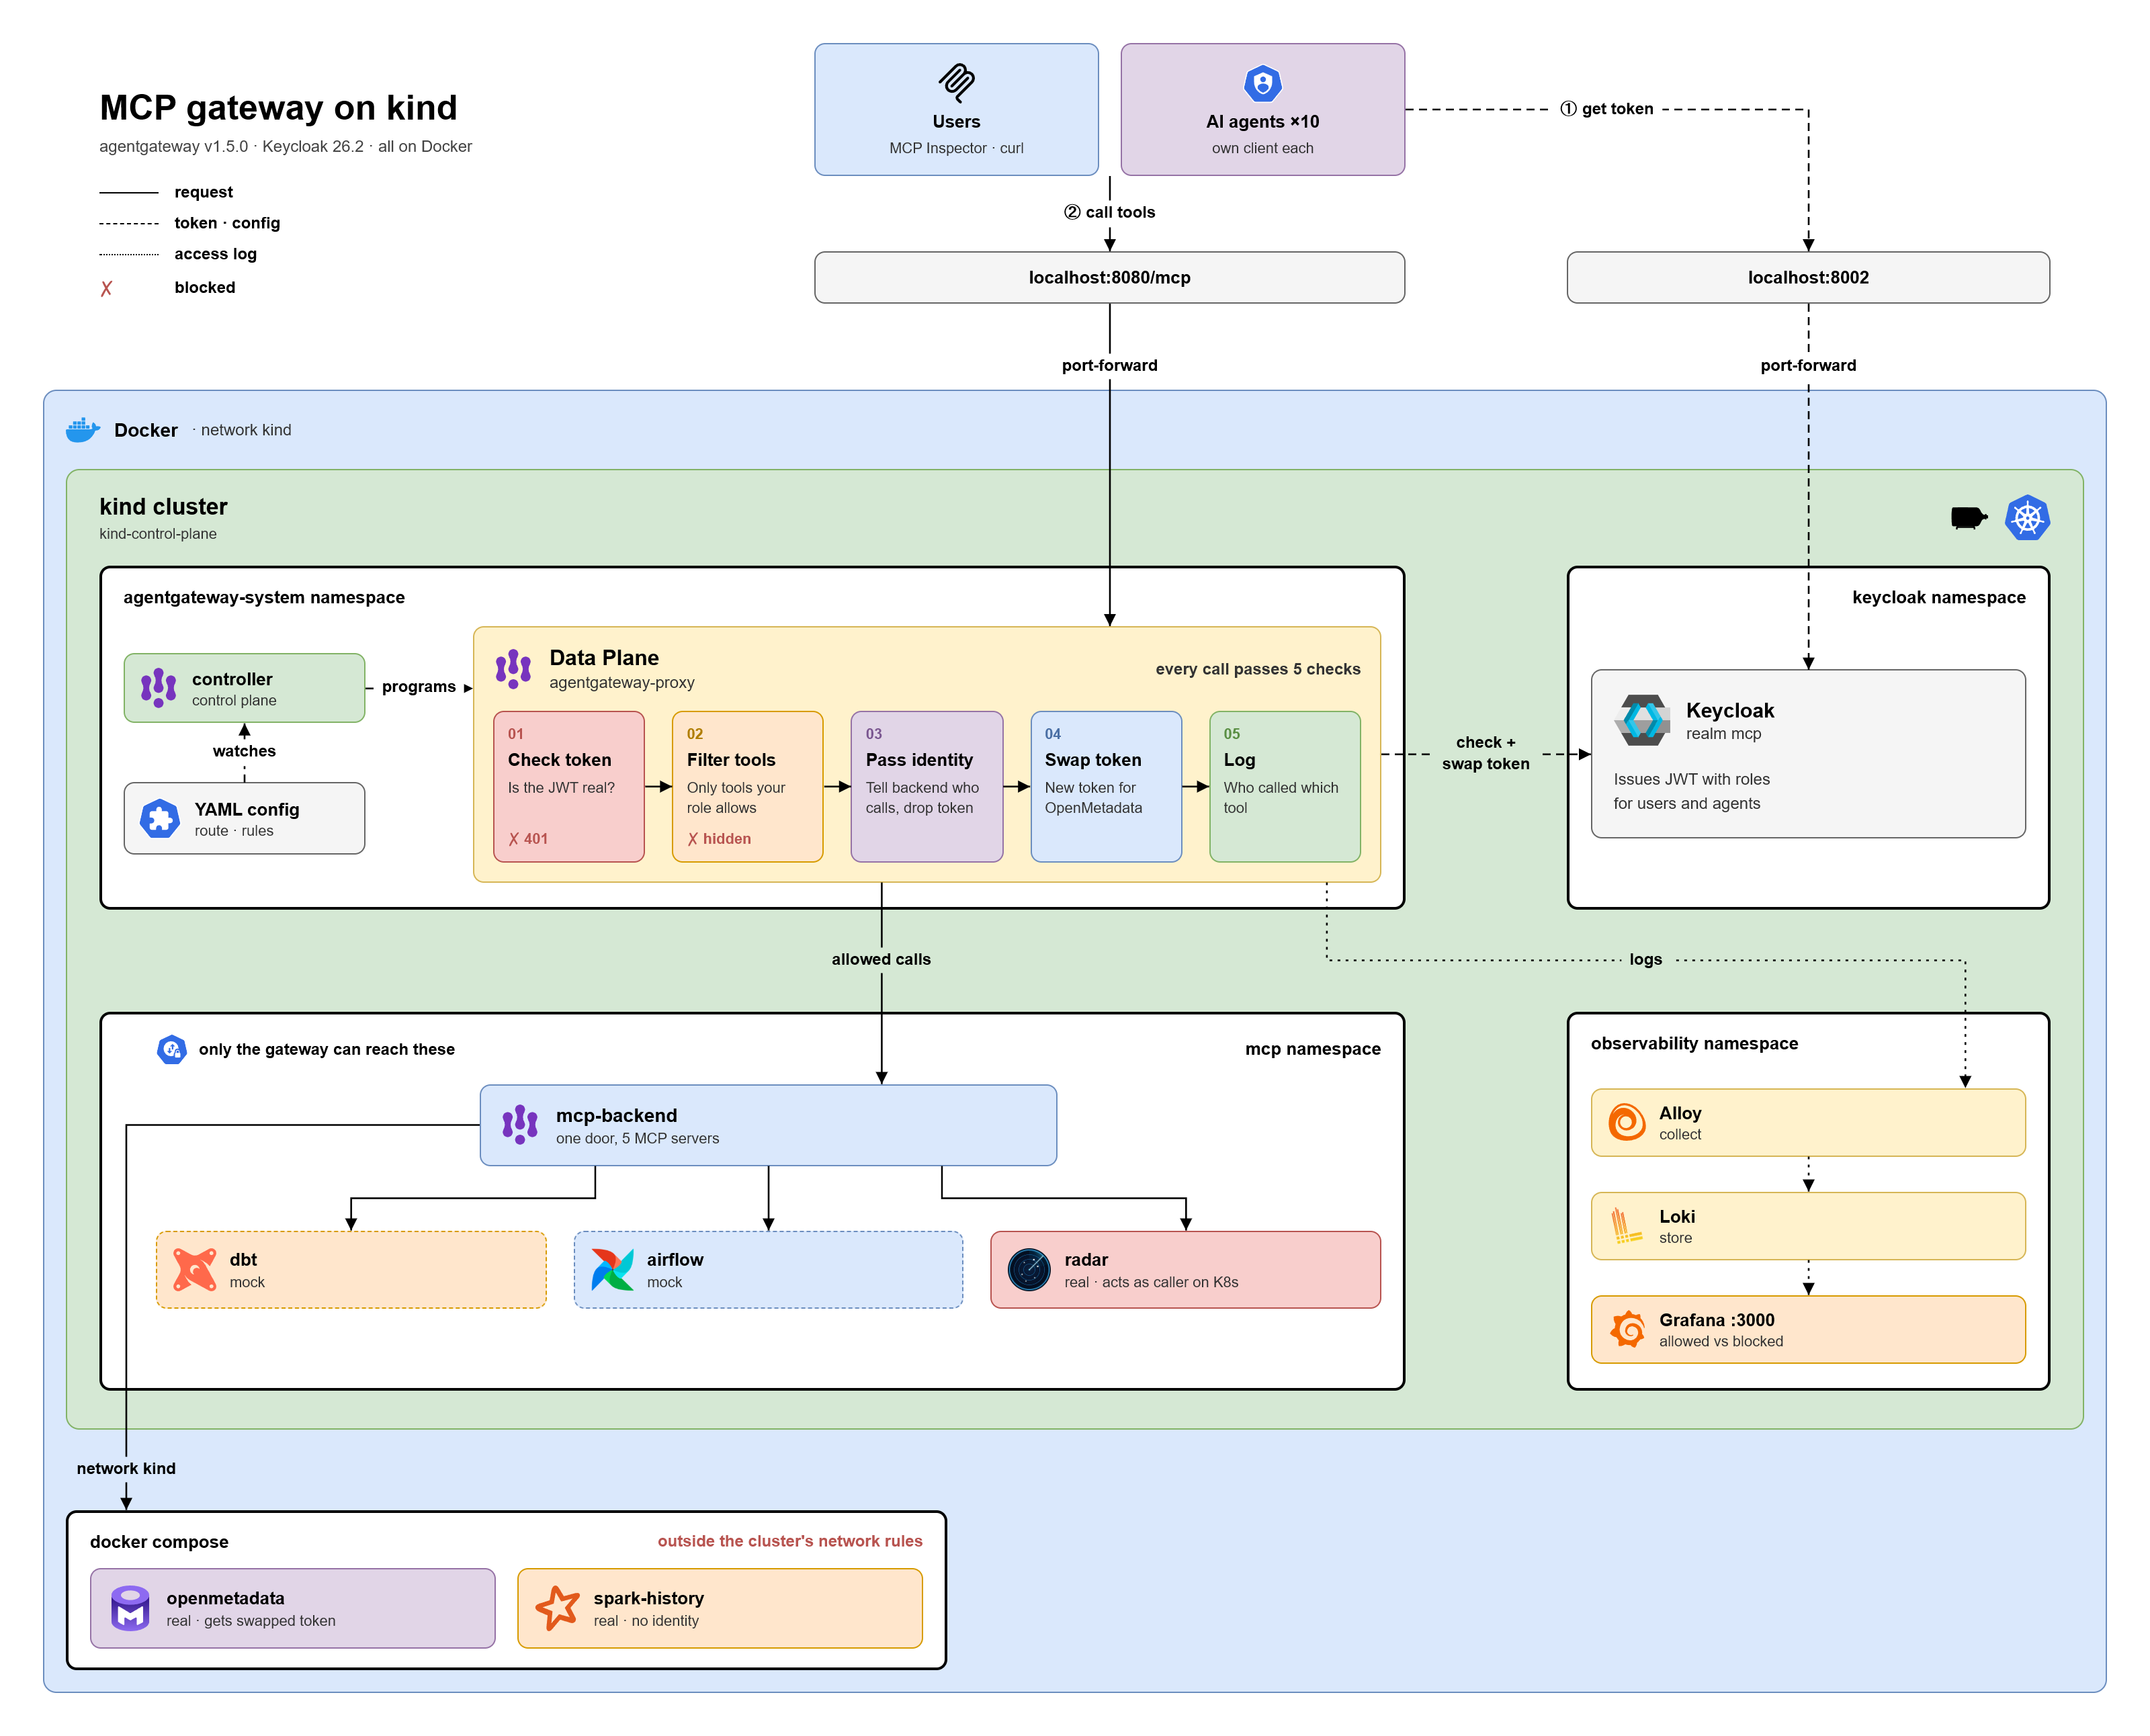
\includegraphics[width=0.85\textwidth]{system-architecture.png}
\caption{Kiến trúc tổng thể hệ thống}\label{fig:arch}\end{figure}

Ở mức triển khai, hệ thống trải trên ba vùng Docker nối với nhau qua network \texttt{kind}: toàn bộ cụm Kubernetes nằm trong một container đóng vai node của kind, còn OpenMetadata và Spark History là hai nhóm container docker compose riêng. Quy tắc mạng ở mục~\ref{sec:netpol} chỉ có hiệu lực trong vùng thứ nhất, nên S4 mới đạt một phần. OpenMetadata gọi ngược vào Keycloak qua NodePort 30802 theo tên node \texttt{gatewayapi-control-plane}, vì vậy tên cụm bị cố định. Ngoài cổng 8080 của gateway, các cổng khác chỉ phục vụ quản trị, gỡ lỗi hoặc dùng nội bộ. Keycloak dùng \texttt{emptyDir} nên mỗi lần dựng lại cụm lại có khóa ký mới, trong khi OpenMetadata dùng volume có tên và giữ cấu hình cũ, nên bước cấu hình OpenMetadata luôn phải chạy lại. Script dọn dẹp chỉ xóa cụm kind và để nguyên hai nhóm container compose; hạn chế này được ghi nhận ở Chương 5.

% =====================================================================
\subsection{Luồng xử lý một yêu cầu}

Hình~\ref{fig:seq} mô tả một lệnh gọi công cụ; các số (1) đến (7) khớp với nhãn trên sơ đồ kiến trúc. Ở bước (1), agent xin token từ Keycloak theo luồng client credentials; token cho biết dịch vụ đích (\texttt{aud = mcp-gateway}), client đang giữ nó (\texttt{azp}) và vai trò (\texttt{roles}). Ở bước (2), agent gửi yêu cầu tới \texttt{/mcp} kèm token.

\begin{figure}[!htb]\centering
\begin{tikzpicture}[font=\small,yscale=0.6,
  tac/.style={draw,fill=gray!10,minimum width=2.3cm,minimum height=8mm,align=center},
  tn/.style={mui},tl/.style={mui,dashed}]
\foreach \x/\n/\t in {0/c/{AI Agent},3.3/k/Keycloak,6.6/g/agentgateway,9.9/b/{MCP backend},13.2/o/{Loki /\\ Grafana}}
  {\node[tac] (\n) at (\x,0) {\t}; \draw[gray] (\n.south) -- ++(0,-12.2);}
\newcommand{\msg}[5]{\draw[#5] (#1,#3) -- node[above,nhan]{#4} (#2,#3);}
\msg{0}{3.3}{-1.2}{(1) xin token}{tn}
\msg{3.3}{0}{-2.0}{JWT: aud, azp, roles}{tl}
\msg{0}{6.6}{-2.8}{(2) POST /mcp + Bearer token}{tn}
\draw[mui] (6.6,-3.4) -- ++(0.6,0) |- node[right,nhan,pos=0.25]{(3) xác thực JWT\\(JWKS, cache 5 phút)} (6.65,-4.4);
\draw[mui] (6.6,-4.9) -- ++(0.6,0) |- node[right,nhan,pos=0.25]{(4) RBAC theo tool\\(CEL, deny-by-default)} (6.65,-5.9);
\draw[mui] (6.6,-6.4) -- ++(0.6,0) |- node[right,nhan,pos=0.25]{(5) đặt header định danh,\\xóa token gốc} (6.65,-7.4);
\msg{6.6}{9.9}{-8.3}{tools/call (không có token)}{tn}
\msg{9.9}{6.6}{-9.1}{kết quả}{tl}
\msg{6.6}{0}{-9.9}{kết quả / lỗi ``Unknown tool''}{tl}
\msg{6.6}{13.2}{-10.9}{(7) access log: user, roles, tool, status}{tn}
\node[nhan,fill=white,draw,dashed] at (8.25,-11.7) {(6) riêng OpenMetadata: token exchange trước bước gửi};
\end{tikzpicture}
\caption{Sơ đồ tuần tự của một lệnh gọi công cụ}\label{fig:seq}\end{figure}

Bước (3) đến (5) diễn ra trong gateway theo thứ tự không được đảo: kiểm tra chữ ký token, kiểm tra quyền dùng công cụ, rồi mới ghi danh tính vào header, xóa token gốc và chuyển tiếp, đúng nguyên tắc ở Chương 3 rằng phân quyền chỉ có nghĩa khi đứng sau một bước xác thực đáng tin. Nếu header được ghi trước khi kiểm tra token, kẻ tấn công có thể tự điền danh tính giả; nếu token bị xóa trước bước (6), OpenMetadata không còn token để đổi. Bước (6) chỉ áp dụng cho OpenMetadata, backend duy nhất tự kiểm tra token: gateway đổi token gốc lấy token có audience riêng để OpenMetadata tự áp quyền theo người gọi. Bước này đã có trong cấu hình nhưng chưa có bằng chứng kiểm thử, nên vẫn thuộc phần chưa hoàn tất.

Hình~\ref{fig:decision} bổ sung các nhánh bị từ chối. Token không hợp lệ nhận HTTP 401; lệnh gọi công cụ không có quyền nhận HTTP 400 kèm \texttt{Unknown tool}, tức công cụ bị coi như không tồn tại. Cách phản hồi này không để lộ công cụ nào có thật, nhưng làm lỗi phân quyền trông giống lỗi gõ sai tên; mục~\ref{sec:obs} trình bày cách xử lý hệ quả đó ở phía giám sát.

\begin{figure}[!htb]\centering
\begin{tikzpicture}[node distance=3.5mm and 10mm]
\node[khoi] (req) {Yêu cầu tới \texttt{/mcp}};
\node[quyetdinh,below=of req] (tok) {Token hợp lệ?};
\node[khoi,right=of tok,fill=red!8] (e401) {HTTP 401};
\node[quyetdinh,below=of tok] (m) {Phương thức?};
\node[khoi,right=of m,xshift=4mm] (list) {Trả danh mục\\đã lọc theo quyền};
\node[quyetdinh,below=of m] (rule) {Có quy tắc\\cho phép?};
\node[khoi,right=of rule,fill=red!8] (e400) {HTTP 400\\``Unknown tool''};
\node[khoi,below=of rule] (hdr) {Đặt header định danh,\\xóa token gốc};
\node[khoi,below=of hdr,fill=green!8] (be) {Chuyển tới backend\\HTTP 200};
\node[khoi,left=18mm of rule] (log) {Ghi access log\\(mọi nhánh)};
\draw[mui] (req) -- (tok);
\draw[mui] (tok) -- node[above,nhan]{không} (e401);
\draw[mui] (tok) -- node[left,nhan]{có} (m);
\draw[mui] (m) -- node[above,nhan]{tools/list} (list);
\draw[mui] (m) -- node[left,nhan]{tools/call} (rule);
\draw[mui] (rule) -- node[above,nhan]{không} (e400);
\draw[mui] (rule) -- node[left,nhan]{có} (hdr);
\draw[mui] (hdr) -- (be);
\draw[dashed,gray,thick] (log.north) |- (tok.west); \draw[dashed,gray,thick] (log.east) -- (rule.west); \draw[dashed,gray,thick] (log.south) |- (be.west);
\end{tikzpicture}
\caption{Lưu đồ quyết định của gateway}\label{fig:decision}\end{figure}

% =====================================================================
\subsection{Các thành phần nền tảng của gateway}\label{sec:netpol}

Mọi yêu cầu tới \texttt{/mcp} được chuyển tới một backend duy nhất của agentgateway chứa năm target. Gateway gộp danh mục của cả năm và gắn tên target vào trước tên công cụ, chẳng hạn \texttt{radar\_list\_namespaces}, qua đó đáp ứng F1 và F2 mà agent không cần biết phía sau có bao nhiêu hệ thống. Đổi lại, tên target trở thành khóa nối mọi thành phần: lệch một ký tự giữa mock, Service, quy tắc phân quyền và bộ kiểm thử là công cụ bị chặn mà không có lỗi nào chỉ ra nguyên nhân. Cấu hình được trích ở Phụ lục B.

Quy tắc xác thực được gắn vào Gateway thay vì vào từng route, để route thêm sau cũng tự động được bảo vệ. Khóa công khai của Keycloak được lưu đệm năm phút, nên khi Keycloak đổi khóa, token mới có thể bị từ chối trong khoảng đó. Sau khi token hợp lệ, gateway \emph{ghi đè} ba header \texttt{x-forwarded-user}, \texttt{x-forwarded-groups} và \texttt{x-agent-id} bằng giá trị lấy từ token, nên mọi header giả do client gửi kèm đều bị thay thế. Token gốc được chuyển tạm sang một header nội bộ để phục vụ việc đổi token cho OpenMetadata, rồi bị một quy tắc thứ hai xóa trước khi yêu cầu rời gateway (S3); thiếu quy tắc này, mọi backend đều nhận được token gốc.

Toàn bộ phân quyền nằm trong một chính sách duy nhất. Mỗi quy tắc là một biểu thức CEL kiểm tra vai trò, target và tên công cụ; các quy tắc được nối bằng phép HOẶC nên người có nhiều vai trò nhận hợp quyền (S2). Như Chương 3 đã chỉ ra, mặc định từ chối chỉ xuất hiện khi backend đã có chính sách \texttt{Allow}, nên chính sách này đồng thời là điều kiện để S1 đứng vững chứ không chỉ là nơi liệt kê quyền. Việc gom vào một chính sách được quyết định sau khi thử nghiệm cho thấy cách gateway kết hợp nhiều chính sách khó dự đoán.

Một NetworkPolicy chỉ cho phép lưu lượng vào namespace backend nếu đến từ namespace của gateway. Đây là mắt xích giữ cho danh tính trong header có giá trị: backend tin \texttt{x-forwarded-user} chỉ vì không pod nào khác gọi thẳng được nó. Hai backend thật chạy bằng Docker nằm ngoài cụm nên không được quy tắc này bảo vệ.

% =====================================================================
\subsection{Mock MCP server và danh mục công cụ}

Kiểm thử phân quyền đòi hỏi gọi từng công cụ với từng vai trò, kể cả công cụ có tác động, điều vừa rủi ro vừa không lặp lại được trên hệ thống thật (mục~\ref{sec:ch3-mock}). Năm mock được viết bằng Python với FastMCP, dùng chung một module (Phụ lục C): server chạy ở chế độ không lưu phiên để bản sao nào của gateway cũng phục vụ được mọi yêu cầu, và mỗi công cụ ghi lại ``ai đang gọi'' gồm ba header danh tính, việc có header \texttt{Authorization} hay không và vài claim không nhạy cảm, không bao giờ ghi bản thân token. Kết quả trả về trong trường \texttt{seen\_by\_mock}, nhờ đó bộ kiểm thử xác nhận từ phía backend rằng danh tính đến đúng người gọi và token gốc đã bị xóa (S3); mức độ đã có bằng chứng được đánh giá ở Chương 5. Cả năm mock dùng chung một image, chạy thành năm Deployment có Service đặt tên đúng bằng tên target.

Mỗi mock mô phỏng các công cụ tiêu biểu với tên và tham số theo MCP server chính thức của phần mềm gốc, để khi chuyển sang phần mềm thật thì quy tắc phân quyền không phải sửa. Danh mục gồm 21 công cụ (Bảng~\ref{tab:tools}; mô tả chi tiết ở Phụ lục C), trong đó 16 công cụ đọc và 5 công cụ ghi hoặc thực thi. Công cụ ghi trong mock không gây tác dụng phụ nên gọi lặp lại được khi kiểm thử; ranh giới đọc/ghi này là nền tảng của thiết kế vai trò.

\begin{table}[H]\centering\caption{Danh mục 21 công cụ theo target và loại}\label{tab:tools}
{\singlespacing\renewcommand{\arraystretch}{1.15}\small
\begin{tabularx}{\textwidth}{|p{2.3cm}|X|p{3.6cm}|}\hline
\textbf{Target} & \textbf{Công cụ đọc} & \textbf{Công cụ ghi / thực thi} \\ \hline
radar & list\_namespaces, list\_resources, get\_pod\_logs & manage\_workload \\ \hline
spark-history & list\_applications, get\_stage, get\_job\_bottlenecks & -- \\ \hline
openmetadata & search\_metadata, get\_entity\_details, get\_entity\_lineage & patch\_entity \\ \hline
dbt & list\_metrics, query\_metrics, get\_model\_health, get\_lineage & test \\ \hline
airflow & list\_dags, get\_dag\_run, get\_task\_logs & trigger\_dag, pause\_dag \\ \hline
\textbf{Tổng} & \textbf{16} & \textbf{5} \\ \hline
\end{tabularx}}\end{table}

% =====================================================================
\subsection{Thiết lập danh tính AI Agent trên Keycloak}\label{sec:agent}

Người dùng đăng nhập bằng mật khẩu và nhận vai trò theo chức danh (\texttt{analyst}, \texttt{bi\_engineer}, \texttt{data\_engineer}, \texttt{data\_admin}). AI Agent không có người đăng nhập, nên mỗi agent là một client riêng trên Keycloak và tự xin token bằng luồng client credentials. Hai loại danh tính được đặt trong cùng một realm và nhận vai trò từ cùng client \texttt{mcp-gateway}, nên gateway chỉ cần một bộ quy tắc thay vì phải tin hai nơi cấp token. Client và vai trò của agent được nạp bằng tính năng nhập một phần (partial import) của Keycloak (Phụ lục D), để phần realm của người dùng được giữ nguyên.

Vai trò của agent được chia theo năng lực trên từng hệ thống thay vì theo chức danh: mỗi hệ thống có mức \textit{viewer} chỉ đọc và mức \textit{operator} hoặc \textit{editor} có thêm thao tác ghi. Agent xử lý sự cố, vốn cần khởi động lại ứng dụng trên Kubernetes và đọc thông tin Spark, chỉ cần ghép \texttt{kube\_operator} với \texttt{spark\_viewer} thay vì nhận vai trò \texttt{data\_engineer} kèm nhiều quyền thừa. Mười agent được tạo, mỗi agent gắn với vai trò năng lực tương ứng (chẳng hạn \texttt{cluster-observer} với \texttt{kube\_viewer}); hai agent phục vụ kiểm chứng hơn là nghiệp vụ: \texttt{no-access} không có vai trò nào để chứng minh mặc định từ chối, còn \texttt{platform-admin} có toàn quyền để chứng minh cả 21 công cụ đều gọi được. Ma trận agent -- vai trò -- công cụ được lưu thành file JSON làm kết quả mong đợi cho bộ kiểm thử ở Chương 5.

Mỗi agent có secret riêng để thu hồi được từng agent; secret dài 256 bit được sinh ngẫu nhiên, ghi thẳng vào Kubernetes Secret, không in ra màn hình và không lưu vào kho mã. Bước sinh secret giữ nguyên secret đã có và dừng lại nếu chỉ một phần tồn tại, vì sinh lại một phần sẽ khiến Kubernetes và Keycloak giữ hai giá trị khác nhau và agent không xin được token.

% =====================================================================
\subsection{Ma trận phân quyền theo vai trò}\label{sec:rolematrix}

Bảng~\ref{tab:rolematrix} tổng hợp quyền của từng vai trò và tổ hợp vai trò trên năm hệ thống; ``Đọc + ghi'' là thêm công cụ ghi hoặc thực thi (Bảng~\ref{tab:tools}). Công cụ không khớp quy tắc nào vừa bị ẩn khỏi danh mục vừa bị từ chối khi gọi.

\begin{table}[H]\centering\caption{Ma trận Vai trò -- Hệ thống -- Công cụ được phép}\label{tab:rolematrix}
{\singlespacing\renewcommand{\arraystretch}{1.15}\setlength{\tabcolsep}{4pt}\small
\begin{tabularx}{\textwidth}{|>{\raggedright\arraybackslash}p{3.3cm}|*{5}{>{\centering\arraybackslash}X|}c|}\hline
\textbf{Vai trò} & \textbf{radar} & \textbf{spark-history} & \textbf{open-\allowbreak metadata} & \textbf{dbt} & \textbf{airflow} & \textbf{Tổng} \\ \hline
\multicolumn{7}{|l|}{\textit{Vai trò người dùng (theo chức danh)}} \\ \hline
analyst & -- & -- & Đọc & -- & -- & 3 \\ \hline
bi\_engineer & -- & -- & Đọc + ghi & -- & -- & 4 \\ \hline
data\_engineer & Đọc & Đọc & Đọc & Đọc & Đọc & 16 \\ \hline
data\_engineer + bi\_engineer & Đọc & Đọc & Đọc + ghi & Đọc & Đọc & 17 \\ \hline
data\_admin & Tất cả & Tất cả & Tất cả & Tất cả & Tất cả & 21 \\ \hline
(không có vai trò) & -- & -- & -- & -- & -- & 0 \\ \hline
\multicolumn{7}{|l|}{\textit{Vai trò của AI Agent (theo năng lực)}} \\ \hline
kube\_viewer & Đọc & -- & -- & -- & -- & 3 \\ \hline
kube\_operator & Đọc + ghi & -- & -- & -- & -- & 4 \\ \hline
spark\_viewer & -- & Đọc & -- & -- & -- & 3 \\ \hline
metadata\_viewer & -- & -- & Đọc & -- & -- & 3 \\ \hline
metadata\_editor & -- & -- & Đọc + ghi & -- & -- & 4 \\ \hline
dbt\_viewer & -- & -- & -- & Đọc & -- & 4 \\ \hline
dbt\_operator & -- & -- & -- & Đọc + ghi & -- & 5 \\ \hline
airflow\_viewer & -- & -- & -- & -- & Đọc & 3 \\ \hline
airflow\_operator & -- & -- & -- & -- & Đọc + ghi & 5 \\ \hline
kube\_operator + spark\_viewer & Đọc + ghi & Đọc & -- & -- & -- & 7 \\ \hline
platform\_admin (khẩn cấp) & Tất cả & Tất cả & Tất cả & Tất cả & Tất cả & 21 \\ \hline
\end{tabularx}}\end{table}

Ma trận vận dụng mô hình RBAC lõi ở Chương 3: mỗi vai trò chỉ nhận công cụ cần cho công việc, công cụ ghi chỉ cấp cho vai trò cần đúng thao tác đó, và các quy tắc nối bằng phép HOẶC nên không cần quy tắc riêng cho từng tổ hợp. Với người dùng, \texttt{analyst} chỉ cần tìm và hiểu dữ liệu nên chỉ đọc OpenMetadata; \texttt{bi\_engineer} chịu trách nhiệm mô tả, gắn thẻ bảng dữ liệu nên được thêm \texttt{patch\_entity}. \texttt{data\_engineer} phải chẩn đoán sự cố xuyên suốt năm hệ thống nên được đọc ở cả năm; ngược lại, cả năm công cụ ghi đều bị giữ lại và phải đi qua \texttt{data\_admin} hoặc agent vận hành chuyên trách. \texttt{data\_admin} không bị giới hạn theo target, nên backend thêm vào sau cũng tự động thuộc quyền quản trị. Token hợp lệ nhưng không mang vai trò nào thì không nhận công cụ nào: xác thực thành công không đồng nghĩa với được phân quyền.

Tổ hợp \texttt{data\_engineer} + \texttt{bi\_engineer} (người dùng \texttt{multi.user}) nhận 17 công cụ, đúng bằng hợp quyền của hai vai trò. Đề tài không dùng quy tắc Deny để giới hạn theo vai trò, vì thí nghiệm chồng lấn chính sách cho thấy Deny được xét theo người dùng chứ không theo vai trò và luôn thắng Allow; nếu chặn radar với \texttt{bi\_engineer}, người giữ cả hai vai trò cũng mất radar dù \texttt{data\_engineer} cho phép. Deny vì vậy chỉ phù hợp với lệnh cấm tuyệt đối. Với agent, mức \textit{operator} hoặc \textit{editor} bao gồm luôn quyền đọc của mức \textit{viewer}, vì agent cần đọc trạng thái trước khi hành động. Tổ hợp \texttt{kube\_operator} + \texttt{spark\_viewer} của agent xử lý sự cố cho 7 công cụ, ít hơn nhiều so với 16 công cụ nếu cấp \texttt{data\_engineer}.

% =====================================================================
\subsection{Tự động hóa triển khai}\label{sec:auto}

Việc dựng môi trường được chia hai giai đoạn theo tần suất thay đổi. Giai đoạn khởi tạo chạy một lần: tạo cụm kind, cài Gateway API, agentgateway và đóng gói image mock, vốn chậm và hiếm khi thay đổi. Cụm dùng để thu bằng chứng ở Chương 5 được tạo theo \path{deploy/cluster/kind-config.yaml}, tắt CNI mặc định và cài Calico. Script khởi tạo \texttt{bootstrap.sh} hiện vẫn tạo cụm với CNI mặc định, nên khi dựng lại bằng script này cần cài Calico theo \path{deploy/cluster/} thì NetworkPolicy mới chắc chắn được thực thi. Giai đoạn khởi động do script up đảm nhiệm, chạy mỗi khi bắt đầu làm việc và chỉ áp lại cấu hình nên nhanh.

Script up gồm ba tầng (Phụ lục E). Tầng ngoài là lớp bọc PowerShell chỉ chuyển đường dẫn sang WSL, gọi hai script bash và đo thời gian, để logic dựng hệ thống chỉ tồn tại ở một nơi. Tầng giữa áp cấu hình theo thứ tự phụ thuộc không đảo được: Keycloak, rồi realm, rồi client của agent và secret của gateway mà việc đổi token cho OpenMetadata cần, sau cùng mới đến phân quyền, NetworkPolicy và access log. Tầng cuối là script giám sát, cài Loki, Alloy, Grafana và chờ cả ba sẵn sàng.

Script được thiết kế idempotent (Chương 3) vì nó hay bị dừng giữa chừng và cách khắc phục đơn giản nhất là chạy lại. Realm chỉ được tạo khi chưa có, vì tạo lại sẽ sinh khóa mới và làm mọi token đang dùng mất hiệu lực; secret của agent cũng chỉ được sinh khi chưa có. Các script bash chạy với \texttt{set -euo pipefail}, nên không báo thành công khi một bước thất bại. Các bước chờ Deployment sẵn sàng đều có giới hạn thời gian, riêng vòng chờ Keycloak trả lời lệnh quản trị chưa có giới hạn và có thể treo nếu Keycloak không lên.

% =====================================================================
\subsection{Giám sát allow/deny}\label{sec:obs}

Access log mặc định của agentgateway không cho biết ai bị chặn ở công cụ nào, nên một quy tắc access log được gắn vào Gateway để ghi thêm sáu trường: tên người dùng, mã agent, danh sách vai trò, phương thức MCP, target và tên công cụ (Phụ lục F). Các trường được lấy từ token đã kiểm tra chứ không từ header do client gửi, để không ai ghi được tên người khác vào log; yêu cầu không có token được ghi là \texttt{anonymous}, và bản thân token không bao giờ được ghi.

Alloy chỉ thu log của các pod \texttt{agentgateway-proxy} và gửi về Loki; Grafana đọc từ Loki và tự nạp dashboard. Bộ ba này đủ nhẹ cho máy cá nhân (mục~\ref{sec:ch3-obs}) và gỡ được mà không ảnh hưởng luồng xử lý chính. Vì gateway không có mã lỗi riêng cho ``không có quyền'' (Hình~\ref{fig:decision}), dashboard phải tự phân loại: lệnh gọi công cụ trả HTTP 200 là cho phép, trả HTTP 400 kèm \texttt{Unknown tool} là bị chặn. Quy tắc này có hai giới hạn. Nó không phân biệt được thiếu quyền với gõ sai tên công cụ, dù trường hợp sau hiếm vì agent lấy tên từ danh mục; và nó phụ thuộc thông báo lỗi của agentgateway 1.5.0, nên cần kiểm tra lại khi nâng cấp. Dashboard có tám ô (Hình~\ref{fig:dashboard}), từ số đếm allow/deny, biểu đồ theo người dùng, vai trò, công cụ đến log từng lệnh gọi, nhờ đó người vận hành trả lời được câu hỏi ``ai đã gọi gì và có bị chặn không'' bằng vài thao tác lọc (O2, S5).

\begin{figure}[!htb]\centering
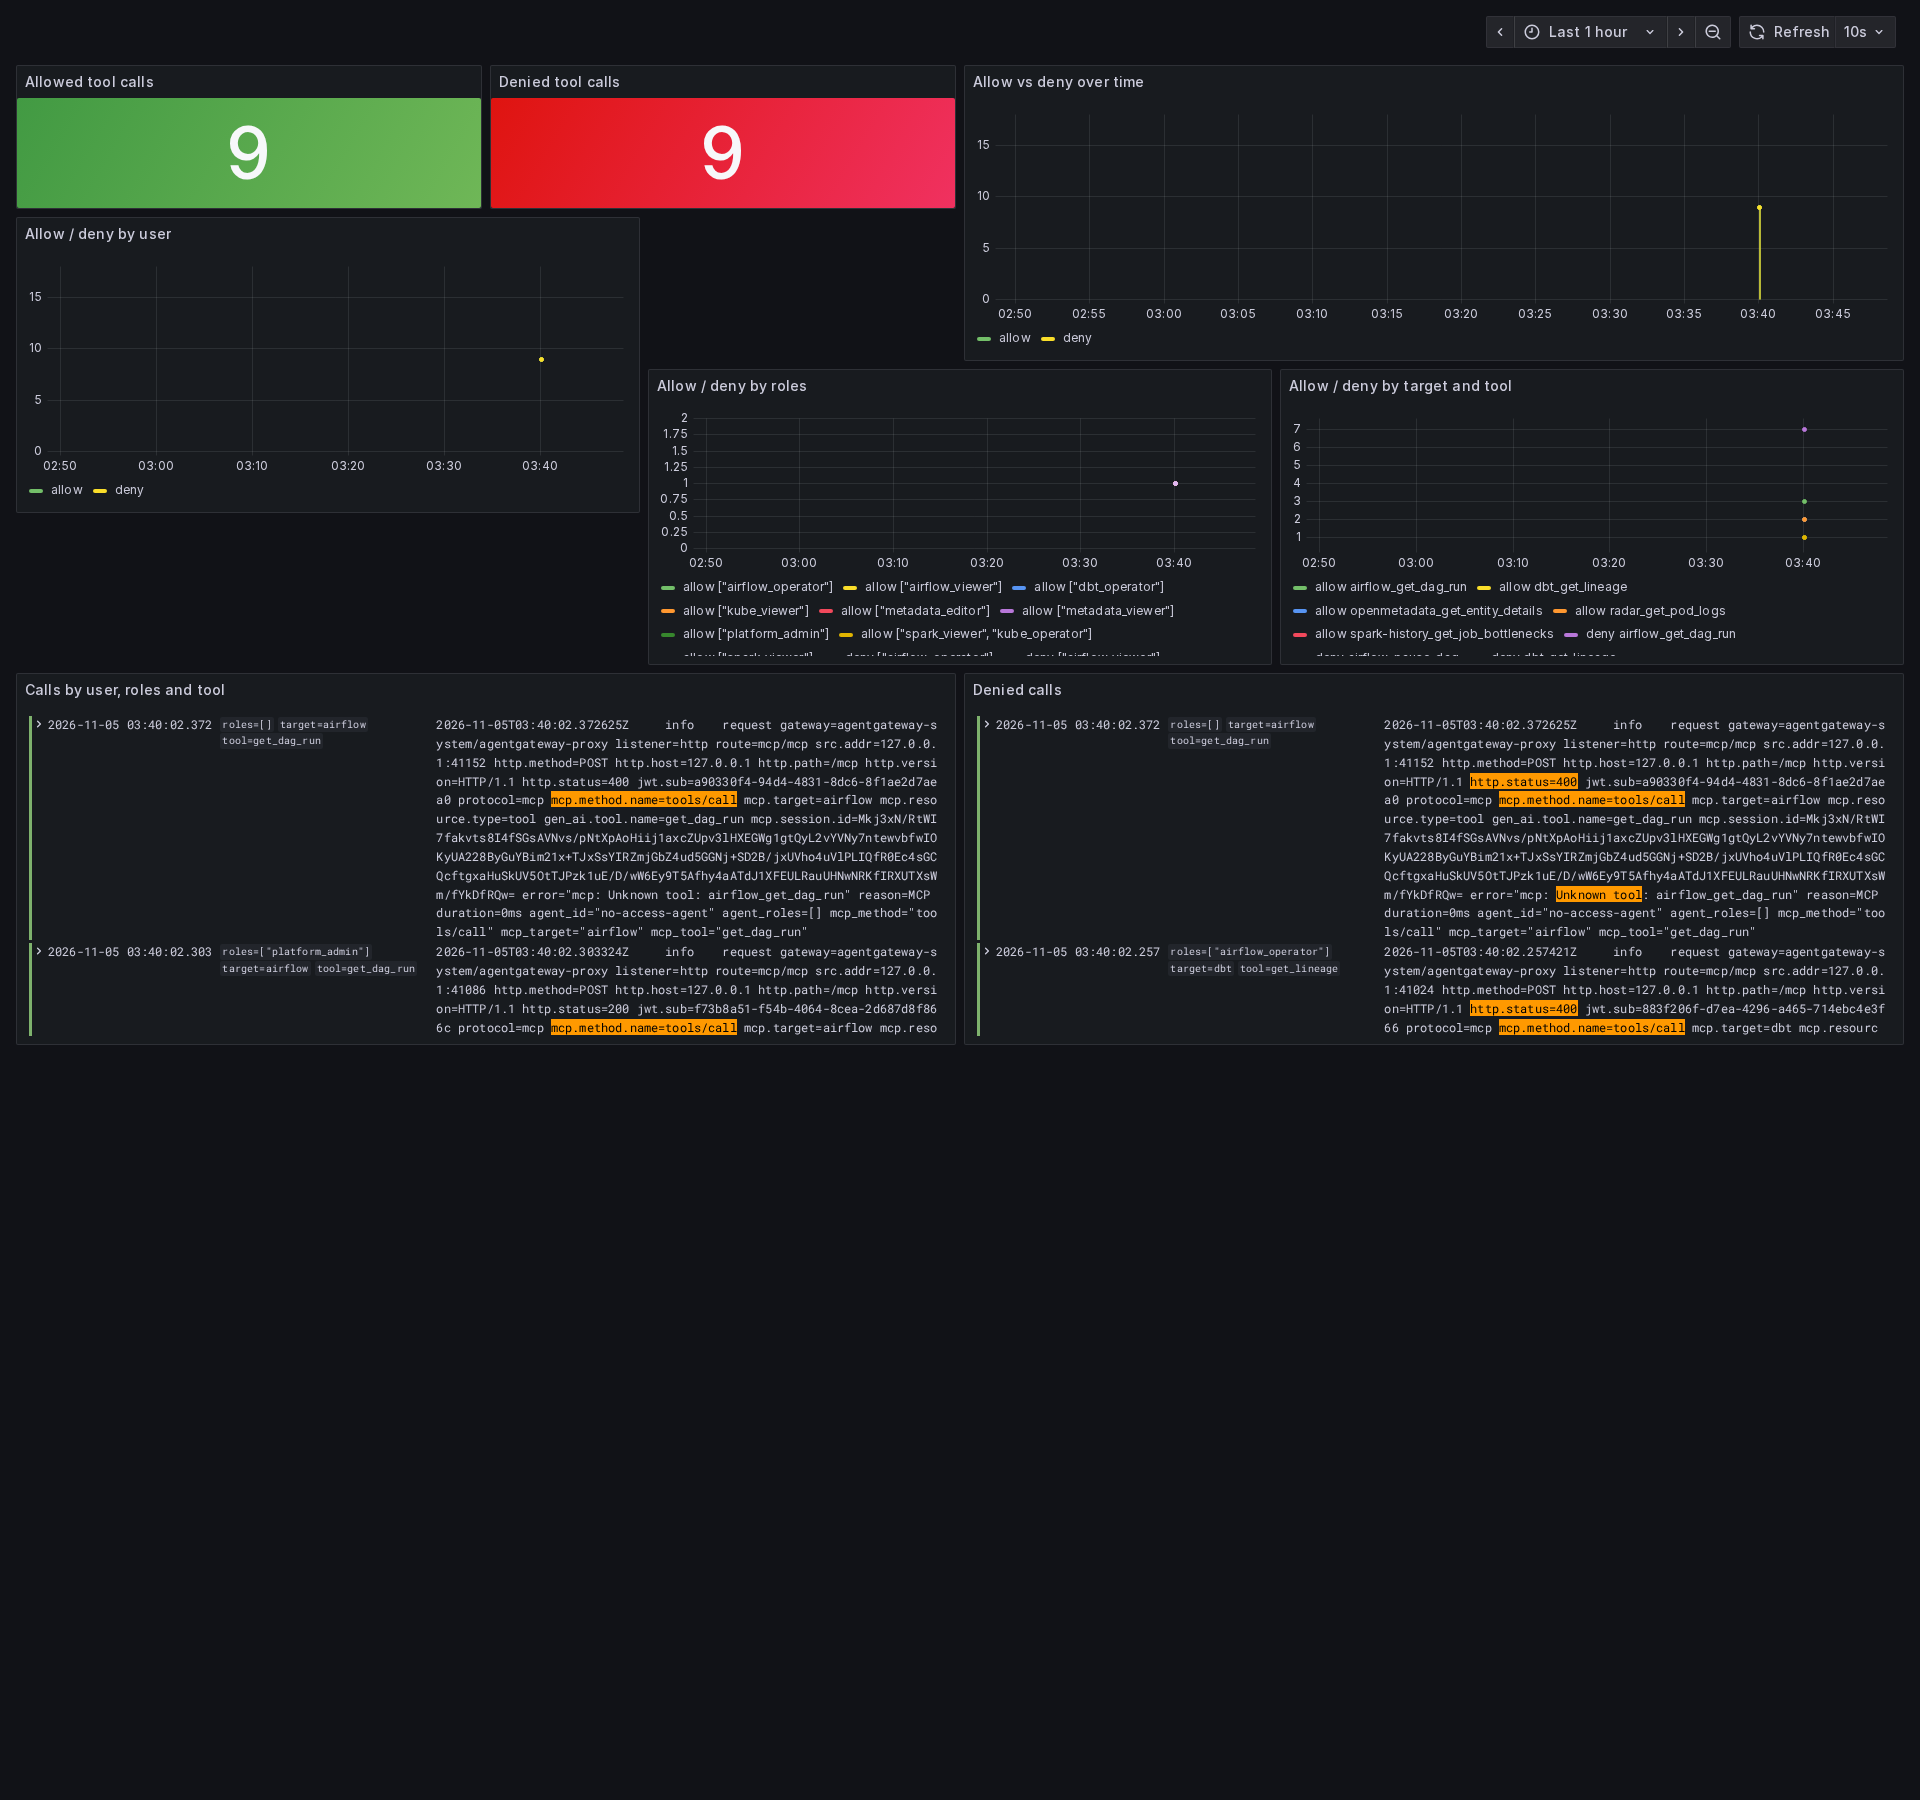
\includegraphics[width=0.75\textwidth,trim=0 750 0 0,clip]{grafana-allow-deny.png}
\caption{Dashboard giám sát allow/deny trên Grafana}\label{fig:dashboard}\end{figure}

\chuong{KIỂM CHỨNG PROOF OF CONCEPT}
\begingroup\setlength{\emergencystretch}{2em}
\subsection{Kịch bản kiểm chứng}

Mỗi yêu cầu ở Bảng~\ref{tab:yeucau} được gắn với ít nhất một kịch bản có tiêu chí đạt xác định trước (Bảng~\ref{tab:scenarios}). Mức tĩnh (K9) đối chiếu ma trận kỳ vọng với danh mục, chính sách và realm mà không cần cụm. Mức đầu cuối gồm hai bộ kiểm thử dùng MCP Python SDK 1.30.0 gọi thật vào \texttt{/mcp} và dừng ở phép so sai đầu tiên, nên ``PASS'' chỉ xuất hiện khi mọi phép so đều đúng.
\begin{table}[H]\centering\caption{Kịch bản kiểm chứng theo yêu cầu}\label{tab:scenarios}
{\singlespacing\renewcommand{\arraystretch}{1.15}\small
\begin{tabularx}{\textwidth}{|c|>{\raggedright\arraybackslash}p{1.5cm}|>{\raggedright\arraybackslash}X|>{\raggedright\arraybackslash}p{4.2cm}|}\hline
\textbf{Mã} & \textbf{Yêu cầu} & \textbf{Kịch bản và tiêu chí đạt} & \textbf{Bằng chứng} \\ \hline
K1 & F1, F2 & Liệt kê và gọi cả 21 công cụ qua \texttt{/mcp}; danh sách tên đã sắp xếp phải trùng khớp và không lệnh nào lỗi & \path{gateway-smoke.txt} (08/10) \\ \hline
K2 & F3, S2 & Mười agent xin token; \texttt{tools/list} của mỗi agent phải trùng ma trận kỳ vọng & \path{agent-rbac-smoke.txt} (29/10) \\ \hline
K3 & S1 & Mỗi agent gọi một công cụ ngoài quyền và phải bị từ chối; ẩn tạm một công cụ rồi gọi thẳng tên của nó & \path{agent-rbac-smoke.txt}, \path{tool-denial*.txt} \\ \hline
K4 & S2, S3 & Token mang đúng \texttt{aud}, \texttt{azp}, \texttt{roles}; backend báo lại đúng header danh tính & \path{agent-rbac-smoke.txt} \\ \hline
K5 & S1, S3 & Gọi bằng curl khi thiếu token, khi gửi header danh tính giả, và kiểm tra token gốc không tới backend & Chưa lưu đầu ra \\ \hline
K6 & S4 & Thăm dò backend radar từ namespace \texttt{default} và từ namespace của gateway & \path{agent-rbac-smoke.txt} \\ \hline
K7 & S5, O2 & Mọi lệnh cho phép và bị chặn phải có bản ghi kèm danh tính agent trong access log và trên dashboard & Access log, ảnh dashboard \\ \hline
K8 & O1 & Năm lần khởi động ấm liên tiếp, mỗi lần kèm kiểm thử phân quyền & \path{benchmarks/warm.md} \\ \hline
K9 & F2, S2 & Kiểm thử tĩnh đối chiếu ma trận, danh mục, chính sách và realm & \path{static_contract_test.mjs} \\ \hline
\end{tabularx}}\end{table}

Môi trường thử là cụm kind một node (Kubernetes v1.37.0, Calico v3.33.0) trên WSL2, cùng agentgateway v1.5.0 và Keycloak 26.2.5, nên kết quả xác nhận tính đúng của cấu hình chứ không cho biết hành vi khi chịu tải hay chạy nhiều node. Bằng chứng được ghi trong ba đợt: 08/10/2026 cho danh mục và thí nghiệm ẩn công cụ, 29/10/2026 cho phân quyền, cô lập mạng và kiểm toán, 05/11/2026 cho dashboard và thời gian khởi động.

\subsection{Kết quả chức năng}

Kịch bản K1 đạt trọn vẹn: gateway trả về 21 công cụ và cả 21 lệnh gọi đều thành công. Vì bộ kiểm thử so toàn bộ danh sách tên đã sắp xếp, một công cụ thiếu, thừa hay sai tiền tố cũng làm lần chạy thất bại; phân bố theo target khớp Bảng~\ref{tab:tools}, tức năm backend được hợp nhất mà không mất hay trùng công cụ nào. Access log cho thấy gateway tách tên đầy đủ trở lại thành target và tên gốc (\texttt{mcp.target=spark-history}, \texttt{gen\_ai.tool.name=get\_stage}), là hai trường mà quy tắc phân quyền đọc.

Lượt chạy này diễn ra trước khi bật JWT, nên access log ghi \texttt{user="anonymous"}. Dưới JWT, danh mục đủ 21 công cụ được xác nhận lại qua \texttt{platform-admin-agent} ở K2 nhưng agent này chỉ gọi một công cụ. F1 và F2 vì vậy có bằng chứng đầy đủ ở bước khám phá, còn bằng chứng gọi đủ 21 công cụ thuộc cấu hình chưa bật xác thực.

\subsection{Kết quả phân quyền}

Cả mười agent đều đạt K2 (Bảng~\ref{tab:rbac}). Do bộ kiểm thử so khớp từng tên chứ không so số lượng, hai cột trùng nhau nghĩa là cả 210 ô của ma trận (10 agent nhân 21 công cụ) đều đúng ở bước khám phá.

\begin{table}[!htbp]\centering\caption{Kết quả kiểm thử phân quyền theo agent}\label{tab:rbac}
{\singlespacing\renewcommand{\arraystretch}{1.15}\small
\begin{tabularx}{\textwidth}{|p{3.6cm}|X|>{\centering\arraybackslash}p{2.4cm}|>{\centering\arraybackslash}p{2.4cm}|}\hline
\textbf{Agent} & \textbf{Vai trò} & \textbf{Được phép} (kỳ vọng/ thực tế) & \textbf{Bị chặn} (kỳ vọng/ thực tế) \\ \hline
cluster-observer & kube\_viewer & 3/3 & 18/18 \\ \hline
incident-response & kube\_operator, spark\_viewer & 7/7 & 14/14 \\ \hline
spark-diagnostic & spark\_viewer & 3/3 & 18/18 \\ \hline
metadata-discovery & metadata\_viewer & 3/3 & 18/18 \\ \hline
metadata-steward & metadata\_editor & 4/4 & 17/17 \\ \hline
dbt-quality & dbt\_operator & 5/5 & 16/16 \\ \hline
airflow-monitor & airflow\_viewer & 3/3 & 18/18 \\ \hline
airflow-operator & airflow\_operator & 5/5 & 16/16 \\ \hline
platform-admin & platform\_admin & 21/21 & 0/0 \\ \hline
no-access & (không có) & 0/0 & 21/21 \\ \hline
\textbf{Tổng (210 ô)} & & \textbf{54/54} & \textbf{156/156} \\ \hline
\end{tabularx}}\end{table}

Hai dòng kiểm tra trực tiếp hai tính chất cốt lõi. \texttt{incident-response-agent}, agent duy nhất mang hai vai trò, nhận đúng 7 công cụ (4 radar cộng 3 Spark), đúng nguyên tắc hợp quyền của S2. \texttt{no-access-agent} thấy danh mục trống dù chính sách không có quy tắc từ chối nào, vì mọi quy tắc cho phép đều gắn với một vai trò; đây là nguyên tắc mặc định từ chối của S1.

Bước gọi (K3) có độ phủ hẹp hơn nhiều: mỗi agent gọi công cụ đầu tiên theo thứ tự chữ cái trong và ngoài quyền, sinh ra 9 lệnh cho phép (trừ \texttt{no-access}) và 9 lệnh bị chặn (trừ \texttt{platform-admin}). Bảy lệnh bị chặn cùng nhắm vào \texttt{airflow\_get\_dag\_run}; chỉ lệnh \texttt{airflow\_pause\_dag} của \texttt{airflow-monitor} thử tách quyền đọc khỏi quyền ghi trên cùng một hệ thống.

Lớp từ chối thứ hai ở bước gọi (Hình~\ref{fig:decision}) được tách riêng trong thí nghiệm ngày 08/10/2026: khi tạm rút quyền với \texttt{airflow\_pause\_dag}, danh mục giảm còn 20 công cụ và lệnh gọi thẳng tên công cụ nhận \texttt{400 Bad Request}; access log ghi \texttt{reason=MCP} cùng \texttt{duration=0ms}, tức gateway tự trả lỗi mà không chuyển xuống backend. Lớp này cần thiết vì một client biết trước tên công cụ không bắt buộc phải đi qua bước khám phá.

\subsection{Kiểm chứng an toàn}

\subsubsection{Token và danh tính}

Chiều chấp nhận của xác thực đã có bằng chứng (K4): token của cả 10 agent mang đúng \texttt{aud}, \texttt{azp} và \texttt{roles}, và ở 9/9 lệnh được phép, mock nhận \texttt{x-agent-id} bằng client ID và \texttt{x-forwarded-user} bằng tên tài khoản dịch vụ tương ứng, tức danh tính lấy từ JWT đã kiểm tra chứ không do client tự điền.

Chiều từ chối chưa có bằng chứng được lưu (K5). Mã 401 khi thiếu token, việc ghi đè header danh tính giả và việc token gốc không tới backend đã được chạy bằng curl nhưng không giữ đầu ra, nên không được tính; token sai chữ ký, sai audience hoặc hết hạn chưa có kịch bản. Riêng S3 có thể khép lại với chi phí nhỏ, vì mock đã báo về trường \texttt{authorization\_present}, chỉ cần bộ kiểm thử khẳng định trường này bằng \texttt{false} trên 9 lệnh được phép.

\subsubsection{Cô lập mạng}

Kịch bản K6 gồm hai lần thăm dò tới backend radar, chỉ có giá trị chứng minh khi đặt cạnh nhau. Kết nối từ namespace \texttt{default} hết thời gian chờ, còn kết nối từ namespace của gateway nhận HTTP 406, mã mà endpoint Streamable HTTP trả về cho một yêu cầu thô không khai báo nhận cả JSON lẫn SSE, nghĩa là backend vẫn chạy và đã trả lời. Riêng lần thứ nhất không loại trừ khả năng backend đang tắt; ghép hai kết quả mới cho thấy backend bị chặn theo nguồn (mục~\ref{sec:netpol}).
\endgroup
\subsection{Kiểm chứng tự động hóa và observability}

Ngày 05/11/2026, bộ đo được lặp năm lần khi cụm và mọi image đã có sẵn, tương ứng tình huống khởi động hằng ngày; mỗi lần áp toàn bộ cấu hình, chờ gateway, Keycloak và Grafana phản hồi, chạy trọn bộ kiểm thử phân quyền rồi đếm lệnh trong access log (Bảng~\ref{tab:bench}).

\begin{table}[!htbp]\centering\caption{Kết quả đo khởi động ấm và kiểm thử phân quyền qua năm lần chạy}\label{tab:bench}
{\singlespacing\renewcommand{\arraystretch}{1.15}\small
\begin{tabularx}{\textwidth}{|X|>{\centering\arraybackslash}p{1.6cm}|>{\centering\arraybackslash}p{1.6cm}|>{\centering\arraybackslash}p{1.6cm}|>{\centering\arraybackslash}p{1.9cm}|}\hline
\textbf{Chỉ số (n = 5)} & \textbf{Nhỏ nhất} & \textbf{Trung bình} & \textbf{Lớn nhất} & \textbf{Độ lệch chuẩn} \\ \hline
Áp cấu hình và cài giám sát (giây) & 4,114 & 4,148 & 4,199 & 0,034 \\ \hline
Đến khi các dịch vụ phản hồi (giây) & 5,142 & 5,177 & 5,230 & 0,036 \\ \hline
Kiểm thử phân quyền 10 agent (giây) & 1,864 & 1,896 & 1,931 & 0,026 \\ \hline
Lệnh cho phép / bị chặn trong access log & 9 / 9 & 9 / 9 & 9 / 9 & 0 \\ \hline
Lần kiểm thử phân quyền đạt & \multicolumn{4}{c|}{5/5} \\ \hline
\end{tabularx}}\end{table}

Độ lệch chuẩn dưới 1\% giá trị trung bình nên kết quả ổn định trong điều kiện đo; hệ thống sẵn sàng phục vụ agent sau khoảng 5,2 giây và một lượt kiểm chứng toàn bộ ma trận quyền mất thêm chưa tới 2 giây. Các con số thấp vì mọi tài nguyên đã tồn tại: \texttt{kubectl apply} chỉ xác nhận trạng thái không đổi, realm và secret của agent được giữ nguyên. Việc năm lần liên tiếp đều đạt kiểm thử phân quyền là bằng chứng cho tính idempotent của script, vì chạy lại không làm đổi danh tính hay khóa ký nên token đang dùng vẫn hợp lệ.
Access log ở cả năm lần ghi đúng 9 lệnh cho phép và 9 lệnh bị chặn, khớp dự đoán của K3, và dashboard hiển thị cùng số liệu (Hình~\ref{fig:allowdeny}). Ở các ô chi tiết (Hình~\ref{fig:dashboard}), lệnh bị chặn của \texttt{no-access-agent} xuất hiện với \texttt{agent\_roles=[]}, \texttt{http.status=400} và \texttt{Unknown tool}, còn lệnh của \texttt{platform-admin-agent} trên cùng công cụ ghi \texttt{http.status=200}. Người vận hành vì vậy xác định được ai gọi, gọi gì và kết quả ra sao mà token không xuất hiện trong log, đúng khả năng kiểm toán S5 và O2 yêu cầu.

\begin{figure}[!htbp]\centering
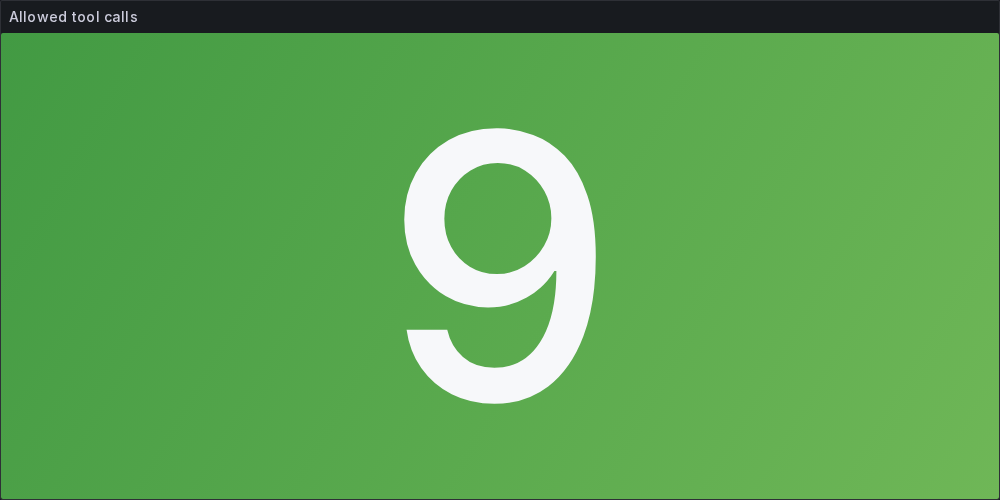
\includegraphics[width=0.4\textwidth]{grafana-allow.png}\hspace{1em}

\includegraphics[width=0.4\textwidth]{grafana-deny.png}
\caption{Số lệnh cho phép và bị chặn trên dashboard sau một lượt kiểm thử}\label{fig:allowdeny}\end{figure}

\begingroup\setlength{\emergencystretch}{2em}
\subsection{Đánh giá}
\subsubsection{Đối chiếu mục tiêu}

Một yêu cầu được xếp ``Đạt'' khi mọi phép đo đã chạy bằng kỳ vọng và phần cốt lõi có đầu ra đã lưu; ``Một phần'' khi các phép đo đã chạy đều đạt nhưng còn tình huống chưa có đầu ra hoặc ngoài phạm vi thử (Bảng~\ref{tab:ch5-goals}).

\begin{table}[H]\centering\caption{Tổng hợp kết quả đo theo yêu cầu}\label{tab:ch5-goals}
{\singlespacing\renewcommand{\arraystretch}{1.15}\small
\begin{tabularx}{\textwidth}{|c|X|>{\centering\arraybackslash}p{1.7cm}|>{\centering\arraybackslash}p{1.7cm}|>{\centering\arraybackslash}p{1.9cm}|}\hline
\textbf{Mã} & \textbf{Phép đo} & \textbf{Kỳ vọng} & \textbf{Thực tế} & \textbf{Mức đạt} \\ \hline
F1 & Lệnh gọi thành công qua \texttt{/mcp} & 21 & 21 & Đạt \\ \hline
F2 & Tên công cụ đúng tiền tố target & 21 & 21 & Đạt \\ \hline
F3 & Ô ma trận khớp ở \texttt{tools/list} & 210 & 210 & Đạt \\ \hline
S1 & Lệnh ngoài quyền bị chặn & 9 & 9 & Một phần \\ \hline
S2 & Agent có claim \texttt{roles} đúng & 10 & 10 & Đạt \\ \hline
S3 & Lệnh mà backend nhận token gốc & 0 & chưa lưu & Một phần \\ \hline
S4 & Lần thăm dò mạng cho kết quả đúng & 2 & 2 & Một phần \\ \hline
S5 & Lệnh gọi có bản ghi kiểm toán & 18 & 18 & Đạt \\ \hline
O1 & Lần khởi động ấm đạt kiểm thử (TB 4,15 giây) & 5 & 5 & Một phần \\ \hline
O2 & Lần đếm allow / deny khớp 9 / 9 & 5 & 5 & Đạt \\ \hline
\end{tabularx}}\end{table}

Sáu yêu cầu đạt, bốn đạt một phần, và không phép đo nào lệch kỳ vọng. Bốn yêu cầu đạt một phần đều do thiếu đầu ra hoặc phạm vi hẹp: S1 chưa có đầu ra cho mã 401 và token sai, S3 cho việc xóa token gốc, S4 chưa thăm dò backend ngoài cụm, O1 chưa đo lần dựng từ cụm trống. Phần lõi của đề tài, gồm danh mục hợp nhất, phân quyền theo công cụ và cô lập mạng trong cụm, đã được kiểm chứng; khoảng trống nằm ở chiều từ chối của xác thực, cũng là chiều kẻ tấn công thường thử đầu tiên, nên lớp an toàn chưa thể coi là hoàn chỉnh.

\subsubsection{Điểm mạnh}

Điểm mạnh rõ nhất là ma trận kỳ vọng được viết thành dữ liệu và dùng chung cho kiểm thử đầu cuối lẫn kiểm thử tĩnh (K9); lần chạy lại kiểm thử tĩnh ngày 05/11/2026 vẫn đạt với 21 công cụ và 10 agent, nên một thay đổi chính sách không kèm cập nhật ma trận bị phát hiện ngay trên máy cá nhân. Thứ hai, việc từ chối diễn ra sớm và tại gateway: 156 trên 210 ô bị ẩn trước khi mô hình kịp chọn công cụ, còn lệnh cố tình gọi bị chặn với \texttt{duration=0ms}. Thứ ba, mỗi lệnh gọi để lại dấu vết ở nhiều phía độc lập (client, mock, access log, dashboard), nên một phía ghi sai sẽ lộ ra qua chênh lệch với các phía còn lại.

\subsubsection{Hạn chế}

Hạn chế lớn nhất là bằng chứng và cấu hình hiện tại không hoàn toàn trùng nhau. Bằng chứng được ghi khi năm target đều là mock và chính sách chỉ chứa quy tắc của agent; từ đó cấu hình đã gộp quy tắc người dùng và agent, chuyển radar, Spark History và OpenMetadata sang phần mềm thật, lấy \texttt{x-forwarded-user} từ \texttt{preferred\_username} và áp NetworkPolicy cho mọi pod backend, nhưng chưa có đầu ra kiểm thử đầu cuối nào trên cấu hình hợp nhất này. Do mock không gây tác dụng phụ, kết quả chưa cho biết gì về quyền trên tài nguyên thật như namespace, DAG hay thực thể metadata, và việc đổi token cho OpenMetadata chưa có bằng chứng.
Độ phủ ở bước gọi còn mỏng: chỉ 18 lệnh được gọi thật và một lệnh thử tách đọc khỏi ghi. Bộ kiểm thử coi mọi ngoại lệ phía client là ``đã bị chặn'', nên không tự phân biệt được từ chối đúng cách với lỗi kết nối; mã 400 chỉ được xác nhận qua access log và dashboard. Dashboard đếm gộp lệnh thiếu quyền với lệnh sai tên công cụ, vì cả hai cùng nhận \texttt{Unknown tool}. Về vận hành, thời gian dựng từ cụm trống và độ trễ gateway thêm vào mỗi lệnh chưa được đo, lớp bọc PowerShell chưa chạy trực tiếp vì phiên đo chạy trong WSL, script dọn dẹp còn để nguyên hai nhóm container compose, và tracing chưa được cấu hình.

\endgroup

\chuong{KẾT LUẬN VÀ KIẾN NGHỊ}

\subsection{Kết quả đạt được}

Đề tài đã xây dựng, hoàn toàn bằng cấu hình các thành phần mã nguồn mở, một hệ thống chứng minh khái niệm trong đó mọi lệnh gọi công cụ của AI Agent đi qua một điểm truy cập MCP duy nhất. Theo Chương 5, sáu trong mười yêu cầu đạt, bốn yêu cầu đạt một phần, và không phép đo nào cho kết quả sai. Cả 21 công cụ gọi được qua gateway; mười agent nhận đúng vai trò trong token, khớp cả 210 ô của ma trận kỳ vọng, và 9 lệnh gọi ngoài quyền đều bị chặn tại gateway. Pod trong namespace \texttt{default} không kết nối được tới backend. Qua năm lần khởi động ấm, bước áp cấu hình mất trung bình 4,15 giây, kiểm thử phân quyền luôn đạt và access log luôn ghi đúng 9 lệnh cho phép, 9 lệnh bị chặn.

Phần chưa trọn vẹn nằm ở chiều từ chối của xác thực và độ khớp giữa bằng chứng với cấu hình: các trường hợp thiếu token, header giả và xóa token gốc chưa lưu đầu ra; lượt gọi đủ 21 công cụ diễn ra trước khi bật JWT; cấu hình hợp nhất với ba backend thật chưa có đầu ra kiểm thử đầu cuối.

\todo{Quân bổ sung kết quả cá nhân và đối chiếu với mục Đánh giá ở Chương 5.}

\subsection{Bài học kinh nghiệm}

Bài học đầu tiên là cấu hình sai thường không báo lỗi mà lặng lẽ làm hệ thống kém an toàn hơn. Khối biến đổi header đặt lồng nhầm trong khối xác thực JWT khiến Kubernetes từ chối tệp mới nhưng chính sách cũ vẫn chạy, nên header danh tính giả vẫn tới backend; tên công cụ kèm tiền tố target làm công cụ bị ẩn không báo; NetworkPolicy trên kind dùng phần mềm mạng mặc định được chấp nhận nhưng không chặn gì. Cả ba lỗi chỉ lộ ra nhờ kiểm thử đầu cuối, nên kiểm thử theo ma trận kỳ vọng là cơ chế an toàn chính của hệ thống xây bằng cấu hình.

Bài học thứ hai là phải kiểm chứng hành vi của công cụ thay vì suy ra từ tài liệu. Thí nghiệm chồng lấn cho thấy chính sách cho phép của agentgateway được nối bằng phép HOẶC, nhưng chính sách từ chối thắng mọi chính sách cho phép và xét theo người gọi chứ không theo vai trò; nếu chỉ có chính sách từ chối, backend vẫn mở cho mọi token hợp lệ, nên mọi quy tắc được gom vào một chính sách cho phép duy nhất. Bài học thứ ba là vai trò của agent nên chia theo năng lực chứ không theo chức danh: vai trò như \texttt{data\_engineer} cấp thừa quyền cho agent, còn chia theo mức đọc và ghi trên từng hệ thống giữ ma trận đủ đơn giản để kiểm thử tự động.

\subsection{Hướng phát triển}

Trước tiên cần khép các khoảng trống bằng chứng: lưu đầu ra cho chiều từ chối của xác thực, khẳng định tự động rằng backend không nhận token gốc và chạy lại kiểm thử đầu cuối trên cấu hình hợp nhất. Tiếp đó là phân quyền ở mức tài nguyên trên backend thật, bắt đầu từ Kubernetes RBAC theo namespace, và hoàn thiện trao đổi token cho OpenMetadata. Xa hơn là xoay vòng và thu hồi secret của agent, cảnh báo chủ động khi lệnh bị chặn tăng bất thường, đưa kiểm thử vào tích hợp liên tục và mở rộng sang agent hành động thay mặt người dùng.

\subsection{Kiến nghị}

Đối với đơn vị, tôi kiến nghị dùng một điểm truy cập MCP duy nhất ngay từ khi đưa AI Agent vào vận hành, cấp cho mỗi agent danh tính riêng và vai trò theo năng lực, tách quyền ghi khỏi quyền đọc, và yêu cầu mọi thay đổi chính sách đi kèm cập nhật ma trận kỳ vọng. Đối với khoa, tôi kiến nghị bổ sung nội dung thực hành về danh tính và phân quyền cho hệ thống tự động, như OAuth 2.0 giữa máy với máy và kiểm soát truy cập theo vai trò.

\heading{TÀI LIỆU THAM KHẢO}
{\setlength{\parskip}{0pt}\printbibliography[heading=none]}
\heading{PHỤ LỤC}

Phụ lục B đến F trích phần cốt lõi của cấu hình và mã nguồn để người đọc đối chiếu với thiết kế ở Chương 4 mà không cần mở kho mã. Đoạn bị lược bỏ được thay bằng dấu ba chấm; bản đầy đủ của từng tệp nằm trong kho mã công khai nêu ở Phụ lục A.

\subsection*{Phụ lục A. Mã nguồn và dữ liệu}
\phantomsection\addcontentsline{toc}{subsection}{Phụ lục A. Mã nguồn và dữ liệu}
\setcounter{table}{0}\renewcommand{\thetable}{A.\arabic{table}}
\textit{A.1. Kho mã}

Toàn bộ cấu hình, mã mock, bộ kiểm thử và bằng chứng của đề tài được công khai tại \url{https://github.com/QuanVongHuu/MCP-gateway-rbac}, kèm hướng dẫn dựng lại hệ thống trong \texttt{QUICKSTART.md}. Bảng~\ref{tab:repo} cho biết vị trí của từng thành phần được nhắc đến trong báo cáo. Để chạy lại, máy cần kind, kubectl, Helm, Docker có Compose với khoảng 8 GB bộ nhớ, Node.js và Python có gói \texttt{mcp} phiên bản 1.30.0. Trên Windows, \texttt{ops/up.ps1} dựng toàn bộ hệ thống qua WSL và \texttt{ops/down.ps1} xóa cụm; trên Linux, \texttt{scripts/up.sh} đảm nhận phần việc dựng tương ứng.

\begin{table}[H]\centering\caption{Vị trí các thành phần trong kho mã}\label{tab:repo}
{\singlespacing\renewcommand{\arraystretch}{1.15}\small
\begin{tabularx}{\textwidth}{|>{\raggedright\arraybackslash}p{5.2cm}|X|}\hline
\textbf{Đường dẫn} & \textbf{Nội dung} \\ \hline
\path{deploy/agentgateway/} & Gateway, HTTPRoute và backend hợp nhất năm target (Phụ lục B.1) \\ \hline
\path{deploy/auth/jwt.yaml} & Xác thực JWT và chuyển tiếp định danh (Phụ lục B.2) \\ \hline
\path{rbac/tool-access.yaml} & Chính sách phân quyền theo công cụ, nguồn sự thật duy nhất (Phụ lục B.3) \\ \hline
\path{deploy/network/backends.yaml} & NetworkPolicy cô lập backend (Phụ lục B.4) \\ \hline
\path{deploy/keycloak/} & Realm, client của agent và script nạp (Phụ lục D) \\ \hline
\path{servers/} & Năm mock MCP server và module dùng chung (Phụ lục C) \\ \hline
\path{tests/} & Kiểm thử tĩnh, kiểm thử đầu cuối và ma trận kỳ vọng \path{tests/expected/agent-tool-access.json} \\ \hline
\path{evidence/} & Đầu ra kiểm thử đã lược bỏ bí mật, dùng ở Chương 5 \\ \hline
\path{ops/}, \path{scripts/} & Script dựng, dọn dẹp và đo thời gian (Phụ lục E) \\ \hline
\path{observability/} & Access log, Loki, Alloy và dashboard Grafana (Phụ lục F) \\ \hline
\end{tabularx}}\end{table}

\textit{A.2. Ghi chú về dữ liệu}

Toàn bộ dữ liệu trong đề tài là dữ liệu thử. Năm mock trả dữ liệu dựng sẵn cho cả 21 công cụ; các công cụ có tính ghi như \texttt{airflow\_trigger\_dag} hay \texttt{radar\_manage\_workload} chỉ trả về kết quả mô phỏng và không gây tác dụng phụ. Ở cấu hình hiện tại, ba target radar, OpenMetadata và Spark History được trỏ sang phần mềm thật chạy cục bộ, nhưng các hệ thống này cũng chỉ chứa dữ liệu thử: radar đọc chính cụm kind của đề tài, OpenMetadata chứa người dùng thử và một bảng mẫu do script cài đặt tạo ra, còn Spark History đọc ba event log mẫu của dự án gốc. Đề tài không sử dụng dữ liệu nghiệp vụ của đơn vị kiến tập.

Các tệp bằng chứng kiểm thử chỉ lưu đầu ra đã lược bỏ bí mật, do đó không chứa client secret, access token hay claim nhạy cảm. Secret của từng agent được sinh trực tiếp vào Kubernetes Secret mà không in ra màn hình; cấu hình realm chỉ giữ biến giữ chỗ như \texttt{\$\{CLUSTER\_OBSERVER\_AGENT\_SECRET\}}. Tài khoản \texttt{admin}/\texttt{admin} của Keycloak và Grafana, cùng mật khẩu \texttt{password} của người dùng thử, là giá trị mặc định dành riêng cho môi trường thử cục bộ và phải được thay trước khi đưa cấu hình ra khỏi máy cá nhân.

\subsection*{Phụ lục B. Cấu hình gateway}
\phantomsection\addcontentsline{toc}{subsection}{Phụ lục B. Cấu hình gateway}
\textit{B.1. Backend hợp nhất năm target}

Cả năm target được khai báo trong một backend duy nhất. Giá trị \texttt{Always} của \texttt{prefixMode} gắn tên target vào trước tên công cụ, tạo ra dạng \texttt{\{target\}\_\{tool\}}. Bốn target còn lại có khai báo giống \texttt{dbt}, chỉ khác tên và địa chỉ.
\begin{lstlisting}
kind: AgentgatewayBackend
spec:
  mcp:
    prefixMode: Always          # tools appear as {target}_{tool}
    targets:
    - name: dbt
      static: {host: dbt.mcp.svc.cluster.local, port: 80, path: /mcp,
               protocol: StreamableHTTP}
    ...
\end{lstlisting}
\textit{B.2. Xác thực JWT và chuyển tiếp định danh}

Chính sách gắn vào Gateway kiểm tra token, ghi đè ba header danh tính bằng claim đã được xác minh, rồi chuyển token gốc từ header \texttt{Authorization} sang header nội bộ \texttt{x-caller-token}. Chính sách thứ hai, gắn vào backend, xóa header nội bộ này trước khi yêu cầu rời gateway (S3).
\begin{lstlisting}
traffic:
  jwtAuthentication:
    mode: Strict
    preserveToken: true
    providers:
    - issuer: http://localhost:8002/realms/mcp
      audiences: [mcp-gateway]
      jwks: {remote: {jwksPath: /realms/mcp/protocol/openid-connect/certs,
                      cacheDuration: "5m", ...}}
  transformation:
    request:
      set:
      - {name: x-forwarded-user,   value: "jwt.preferred_username"}
      - {name: x-agent-id,         value: "has(jwt.azp) ? jwt.azp : ''"}
      - {name: x-forwarded-groups, value: "has(jwt.roles) ? jwt.roles.join(',') : ''"}
      - {name: x-caller-token,     value: 'request.headers["authorization"]'}
      remove: [authorization]
---
# second policy, on the backend: drop the token before it leaves the gateway
backend: {transformation: {request: {remove: [x-caller-token]}}}
\end{lstlisting}
\textit{B.3. Phân quyền theo công cụ}

Toàn bộ quy tắc nằm trong một chính sách \texttt{Allow} duy nhất. Các biểu thức được kết hợp bằng phép HOẶC, nên agent có nhiều vai trò nhận hợp các quyền; công cụ không khớp biểu thức nào bị ẩn khỏi danh mục và bị từ chối khi gọi.
\begin{lstlisting}
backend:
  mcp:
    authorization:
      action: Allow
      policy:
        matchExpressions:      # expressions are OR-ed
        - 'has(jwt.roles) && "analyst" in jwt.roles
           && mcp.tool.target == "openmetadata"
           && mcp.tool.name in ["search_metadata", "get_entity_details", ...]'
        ...
        - 'has(jwt.roles) && "kube_operator" in jwt.roles
           && mcp.tool.target == "radar" && mcp.tool.name == "manage_workload"'
        - 'has(jwt.roles) && "platform_admin" in jwt.roles'
\end{lstlisting}
\textit{B.4. Cô lập mạng}

Chính sách áp dụng cho mọi pod trong namespace \texttt{mcp} và chỉ cho phép kết nối đến từ namespace của gateway (S4).
\begin{lstlisting}
kind: NetworkPolicy
metadata: {name: backends-from-gateway-only, namespace: mcp}
spec:
  podSelector: {}               # every pod in namespace mcp
  policyTypes: [Ingress]
  ingress:
  - from:
    - namespaceSelector:
        matchLabels: {kubernetes.io/metadata.name: agentgateway-system}
\end{lstlisting}

\subsection*{Phụ lục C. Mock MCP server}
\phantomsection\addcontentsline{toc}{subsection}{Phụ lục C. Mock MCP server}
\textit{C.1. Bộ khung chung}
\begin{lstlisting}[language=Python]
def new_server(name):
    # stateless + JSON: any gateway replica can serve any request
    return FastMCP(name, host="0.0.0.0", port=8000,
                   stateless_http=True, json_response=True)

def seen(ctx, target, tool, args):
    """Log who called which tool. Never logs the token itself."""
    headers = ctx.request_context.request.headers
    record = {"target": target, "tool": tool, "args": args,
              "x_agent_id": headers.get("x-agent-id"),
              "x_forwarded_user": headers.get("x-forwarded-user"),
              "x_forwarded_groups": headers.get("x-forwarded-groups"),
              "authorization_present": "authorization" in headers}
    if token := bearer(headers):          # non-sensitive claims only
        claims = decode(token)
        record["token"] = {k: claims.get(k) for k in
                           ("iss", "aud", "azp", "sub", "preferred_username", "roles")}
    print(json.dumps(record))
    return record
\end{lstlisting}
\textit{C.2. Một công cụ mẫu}
\begin{lstlisting}[language=Python]
@mcp.tool()
def test(ctx, selector=""):
    """EXECUTE: run dbt data tests. Mock: nothing is run."""
    who = seen(ctx, "dbt", "test", {"selector": selector})
    return {"result": "mock: dbt test -> PASS=17 WARN=1 ERROR=1",
            "seen_by_mock": who}
\end{lstlisting}
\textit{C.3. Chức năng của 21 công cụ}
{\singlespacing\renewcommand{\arraystretch}{1.2}\small
\begin{longtable}{|p{2.4cm}|p{3.8cm}|c|p{6.4cm}|}\hline
\textbf{Target} & \textbf{Công cụ} & \textbf{Loại} & \textbf{Chức năng} \\ \hline\endhead
radar & list\_namespaces & Đọc & Liệt kê namespace của cụm \\ \hline
radar & list\_resources & Đọc & Tóm tắt tài nguyên theo loại \\ \hline
radar & get\_pod\_logs & Đọc & Lấy log gần nhất của pod \\ \hline
radar & manage\_workload & Ghi & Khởi động lại, scale, rollback workload \\ \hline
spark-history & list\_applications & Đọc & Liệt kê ứng dụng Spark theo trạng thái \\ \hline
spark-history & get\_stage & Đọc & Chi tiết một stage và chỉ số task \\ \hline
spark-history & get\_job\_bottlenecks & Đọc & Tìm stage chậm, task lệch, lỗi executor \\ \hline
openmetadata & search\_metadata & Đọc & Tìm tài sản dữ liệu theo từ khóa, owner, tag \\ \hline
openmetadata & get\_entity\_details & Đọc & Chi tiết một thực thể theo tên đầy đủ \\ \hline
openmetadata & get\_entity\_lineage & Đọc & Nguồn phía trên và đích phía dưới \\ \hline
openmetadata & patch\_entity & Ghi & Sửa mô tả, tag, owner bằng JSON Patch \\ \hline
dbt & list\_metrics & Đọc & Liệt kê metric của semantic layer \\ \hline
dbt & query\_metrics & Đọc & Truy vấn metric theo chiều \\ \hline
dbt & get\_model\_health & Đọc & Trạng thái chạy, test, độ tươi của model \\ \hline
dbt & get\_lineage & Đọc & Cha và con của một node \\ \hline
dbt & test & Thực thi & Chạy data test theo selector \\ \hline
airflow & list\_dags & Đọc & Liệt kê DAG và lần chạy gần nhất \\ \hline
airflow & get\_dag\_run & Đọc & Trạng thái một lần chạy DAG \\ \hline
airflow & get\_task\_logs & Đọc & Log của một lần thử task \\ \hline
airflow & trigger\_dag & Ghi & Kích hoạt một lần chạy mới \\ \hline
airflow & pause\_dag & Ghi & Tạm dừng DAG \\ \hline
\end{longtable}}

\subsection*{Phụ lục D. Danh tính AI Agent}
\phantomsection\addcontentsline{toc}{subsection}{Phụ lục D. Danh tính AI Agent}
\textit{D.1. Định nghĩa một client agent}
\begin{lstlisting}
{"clientId": "cluster-observer-agent",
 "publicClient": false, "serviceAccountsEnabled": true,
 "standardFlowEnabled": false, "directAccessGrantsEnabled": false,
 "secret": "${CLUSTER_OBSERVER_AGENT_SECRET}",
 "protocolMappers": [ audience mcp-gateway, client roles -> claim "roles",
                      hardcoded claim kube_group = "kube_viewer" ]}
...
"users": [{"serviceAccountClientId": "cluster-observer-agent",
           "clientRoles": {"mcp-gateway": ["kube_viewer"]}}, ...]
\end{lstlisting}
\textit{D.2. Nạp agent vào realm}
\begin{lstlisting}[language=bash]
for cid in <clients with a secret>; do   # replace placeholders with real secrets
  sec=$(kubectl get secret agent-client-secrets -o jsonpath={.data.$cid} | base64 -d)
  json=$(jq '(.clients[] | select(.clientId == $c)).secret = $s' ...)
done
# partial import: agent clients and roles only, mcp-gateway untouched
kcadm.sh create partialImport -r mcp  (ifResourceExists: OVERWRITE)
kcadm.sh add-roles --uusername service-account-$cid --rolename $role
\end{lstlisting}

\subsection*{Phụ lục E. Tự động hóa triển khai}
\phantomsection\addcontentsline{toc}{subsection}{Phụ lục E. Tự động hóa triển khai}
\textit{E.1. Lớp bọc PowerShell}
\begin{lstlisting}
$repoDir = (& wsl.exe -d $Distro -- wslpath -u $PSScriptRoot).Trim()
$command = "cd '$repoDir' && bash scripts/up.sh && bash observability/grafana/up.sh"
$stopwatch = [System.Diagnostics.Stopwatch]::StartNew()
& wsl.exe -d $Distro -- bash -lc $command
if ($LASTEXITCODE -ne 0) { throw "Startup failed after $($stopwatch.Elapsed)" }
\end{lstlisting}
\textit{E.2. Áp các lớp cấu hình}
\begin{lstlisting}[language=bash]
set -euo pipefail
kubectl apply -f deploy/agentgateway/Gateway.yaml -f servers/k8s/mocks.yaml ...
kubectl apply -f deploy/keycloak/keycloak.yaml
# setup-realm.sh rebuilds the realm, so only run it when the realm is missing
kcadm.sh get realms/mcp || bash deploy/keycloak/setup-realm.sh
bash scripts/bootstrap-agent-secrets.sh && bash deploy/keycloak/setup-agents.sh
kubectl apply -f deploy/auth/jwt.yaml -f deploy/identity/openmetadata.yaml
kubectl apply -f rbac/tool-access.yaml
kubectl apply -f deploy/network/backends.yaml
kubectl apply -f observability/access-logs/policy.yaml
\end{lstlisting}
\textit{E.3. Script dọn dẹp}
\begin{lstlisting}
& kind delete cluster --name $ClusterName
if ($LASTEXITCODE -ne 0) { Write-Error "Failed to delete ..."; exit $LASTEXITCODE }
\end{lstlisting}

\subsection*{Phụ lục F. Giám sát allow/deny}
\phantomsection\addcontentsline{toc}{subsection}{Phụ lục F. Giám sát allow/deny}
\textit{F.1. Bổ sung trường vào access log}
\begin{lstlisting}
frontend:
  accessLog:
    attributes:
      add:
      - {name: user,       expression: 'has(jwt.preferred_username) ? ... : "anonymous"'}
      - {name: agent_id,   expression: 'has(jwt.azp) ? jwt.azp : ""'}
      - {name: roles,      expression: 'has(jwt.roles) ? jwt.roles : []'}
      - {name: mcp_method, expression: 'has(mcp.methodName) ? mcp.methodName : ""'}
      - {name: mcp_target, expression: 'has(mcp.tool.target) ? mcp.tool.target : ""'}
      - {name: mcp_tool,   expression: 'has(mcp.tool.name) ? mcp.tool.name : ""'}
\end{lstlisting}
\textit{F.2. Truy vấn LogQL đếm deny theo vai trò}
\begin{lstlisting}
sum by (roles) (count_over_time(
  {namespace="agentgateway-system"}
  |~ `mcp.method.name=tools/call` |~ `http.status=400` |~ `Unknown tool`
  | regexp `roles=(?P<roles>\[[^]]*\])` [$__interval]))
\end{lstlisting}

\subsection*{Phụ lục G. Phân công trong nhóm}
\phantomsection\addcontentsline{toc}{subsection}{Phụ lục G. Phân công trong nhóm}
\setcounter{table}{0}\renewcommand{\thetable}{G.\arabic{table}}
Bảng~\ref{tab:phancong} trình bày phân công theo từng công việc trong kế hoạch của nhóm. Thời gian ghi trong bảng là thời gian theo kế hoạch, nên có thể lệch vài ngày so với mốc commit được ghi ở Lịch làm việc. Cột ``Tham gia'' ghi tên thành viên hỗ trợ ở những công việc không do mình phụ trách chính.

\begin{table}[H]\centering\caption{Phân công thực hiện}\label{tab:phancong}
{\singlespacing\renewcommand{\arraystretch}{1.2}\small
\begin{tabularx}{\textwidth}{|X|>{\centering\arraybackslash}p{2.5cm}|>{\centering\arraybackslash}p{2.4cm}|>{\centering\arraybackslash}p{1.6cm}|}\hline
\textbf{Công việc} & \textbf{Thời gian} & \textbf{Phụ trách chính} & \textbf{Tham gia} \\ \hline
Dựng MCP Gateway trên Kubernetes & 30/09 -- 02/10 & \multicolumn{2}{c|}{Cả nhóm} \\ \hline
Mock MCP server cho năm backend (21 công cụ) & 05/10 -- 07/10 & Quân & Huy \\ \hline
Khảo sát khả năng quan sát của agentgateway (log, metric, trace, admin UI) & 05/10 -- 07/10 & Huy & -- \\ \hline
Thí nghiệm chồng lấn chính sách phân quyền & 06/10 -- 07/10 & Quân & -- \\ \hline
Realm Keycloak, xác thực JWT và quy tắc phân quyền theo công cụ & 07/10 -- 11/10 & Quân & -- \\ \hline
Dựng và dọn môi trường bằng một lệnh & 06/10 -- 12/10 & \multicolumn{2}{c|}{Quân (bản Linux), Huy (bản Windows)} \\ \hline
Dashboard allow/deny trên Grafana & 09/10 -- 12/10 & Huy & -- \\ \hline
Kiểm chứng lọc danh mục công cụ theo vai trò & 12/10 & Quân & -- \\ \hline
Kiểm chứng từ chối lệnh gọi và các trường hợp biên & 13/10 & Quân & -- \\ \hline
Tổng hợp kết quả giai đoạn 1 vào báo cáo nháp & 12/10 -- 15/10 & Quân & -- \\ \hline
Danh tính AI Agent, cô lập mạng bằng NetworkPolicy và tài liệu bổ sung & 22/10 -- 27/10 & Huy & -- \\ \hline
Hoàn thiện README và tài liệu dự án & 30/10 -- 04/11 & Quân & -- \\ \hline
Viết báo cáo & -- & \multicolumn{2}{c|}{Chia theo chương, đọc chéo} \\ \hline
\end{tabularx}}\end{table}


\end{document}
